% Created 2020-02-10 Mon 18:34
% Intended LaTeX compiler: pdflatex
\documentclass[a4paper, justified, notitlepage, sfsidenotes, notoc]{tufte-book}
     \input{/users/rakhim/.emacs.d/latex/tufte.tex}
\usepackage[utf8]{inputenc}
\usepackage[T1]{fontenc}
\usepackage{graphicx}
\usepackage{grffile}
\usepackage{longtable}
\usepackage{wrapfig}
\usepackage{rotating}
\usepackage[normalem]{ulem}
\usepackage{amsmath}
\usepackage{textcomp}
\usepackage{amssymb}
\usepackage{capt-of}
\usepackage{hyperref}
\date{}
\title{Computer Science For The Busy Developer}
\hypersetup{
 pdfauthor={Rakhim Davletkaliyev},
 pdftitle={Computer Science For The Busy Developer},
 pdfkeywords={},
 pdfsubject={},
 pdfcreator={Emacs 26.3 (Org mode 9.1.9)},
 pdflang={English}}
\begin{document}

\begin{titlepage}
\begin{fullwidth} % Suppresses headers and footers on the title page

	\centering % Centre everything on the title page

	\scshape % Use small caps for all text on the title page

	\vspace*{\baselineskip} % White space at the top of the page

	%------------------------------------------------
	%	Title
	%------------------------------------------------

	\rule{\textwidth}{1.6pt}\vspace*{-\baselineskip}\vspace*{2pt} % Thick horizontal rule
	\rule{\textwidth}{0.4pt} % Thin horizontal rule

	\vspace{0.75\baselineskip} % Whitespace above the title

	{\LARGE COMPUTER SCIENCE\\ FOR\\ THE BUSY DEVELOPER\\} % Title

	\vspace{0.75\baselineskip} % Whitespace below the title

	\rule{\textwidth}{0.4pt}\vspace*{-\baselineskip}\vspace{3.2pt} % Thin horizontal rule
	\rule{\textwidth}{1.6pt} % Thick horizontal rule

	\vspace{2\baselineskip} % Whitespace after the title block

	%------------------------------------------------
	%	Subtitle
	%------------------------------------------------

  A Relatively Quick Overview\\ Of Core Concepts Of Theoretical Computer Science

	\vspace*{3\baselineskip} % Whitespace under the subtitle

	%------------------------------------------------
	%	Editor(s)
	%------------------------------------------------

	DRAFT

	\vspace{0.5\baselineskip} % Whitespace before the editors

	{\scshape\Large Rakhim Davletkaliyev \\} % Editor list

	\vspace{0.5\baselineskip} % Whitespace below the editor list

	\textit{Codexpanse\\ Helsinki, Finland} % Editor affiliation

	\vfill % Whitespace between editor names and publisher logo

	%------------------------------------------------
	%	Publisher
	%------------------------------------------------



	2019 % Publication year

	% {\large publisher} % Publisher

\end{fullwidth}
\end{titlepage}
\setcounter{tocdepth}{4}
\tableofcontents

\part{Intro}
\label{sec:orgb00b7b6}

This course and the book constitute an high speed overview of the most important fundamental computer science areas. It is intended for intermediate and professional developers who, for any reason, are interested in getting to know the formal, academic side of CS better.

The goal is to provide an overview deep enough so that you end up understanding the ares, their problems and the connections between them. And shallow enough so that you aren't buried under hundreds of pages of proofs, formalizations and exercises.

We will start by trying to understand what computer science is and why it isn't a new area at all. We'll consider the computability as a fundamental property of reality rather than a technological apparatus.

We shall then proceed to learning essential mathematics necessary for further topics. These include proof techniques, notation and logic.

Next, we will learn about the following topics:

\begin{enumerate}
\item Set theory.
\item Algorithms. Complexity and examples of important algorithms in sorting.
\item Abstract Data Types.
\item Graph theory.
\item Theory of computation.
\item Cryptography.
\item Information theory.
\end{enumerate}

Since it seems impossible or at least unpractical to put all of computer science curriculum into a single course, even in a minified format, we shall leave the following topics for the last chapter. In it, we will give an overview to them:

\begin{itemize}
\item Abstract algebra
\item Category theory
\item Type theory
\item Computational geometry
\end{itemize}

\part{Foundations of Math}
\label{sec:org0627daf}
\chapter{Set theory}
\label{sec:orgb876989}

\section{Intro to sets}
\label{sec:org99a5758}

\textbf{\textbf{Set theory}} is an important area of math which lays as a foundation of many computer science topics, such as databases and types in programming. Set theory isn't difficult conceptually, and is generally nice to think about, especially if you like to visualize.

A \textbf{\textbf{set}} is simply a collection of things.

\begin{marginfigure}
  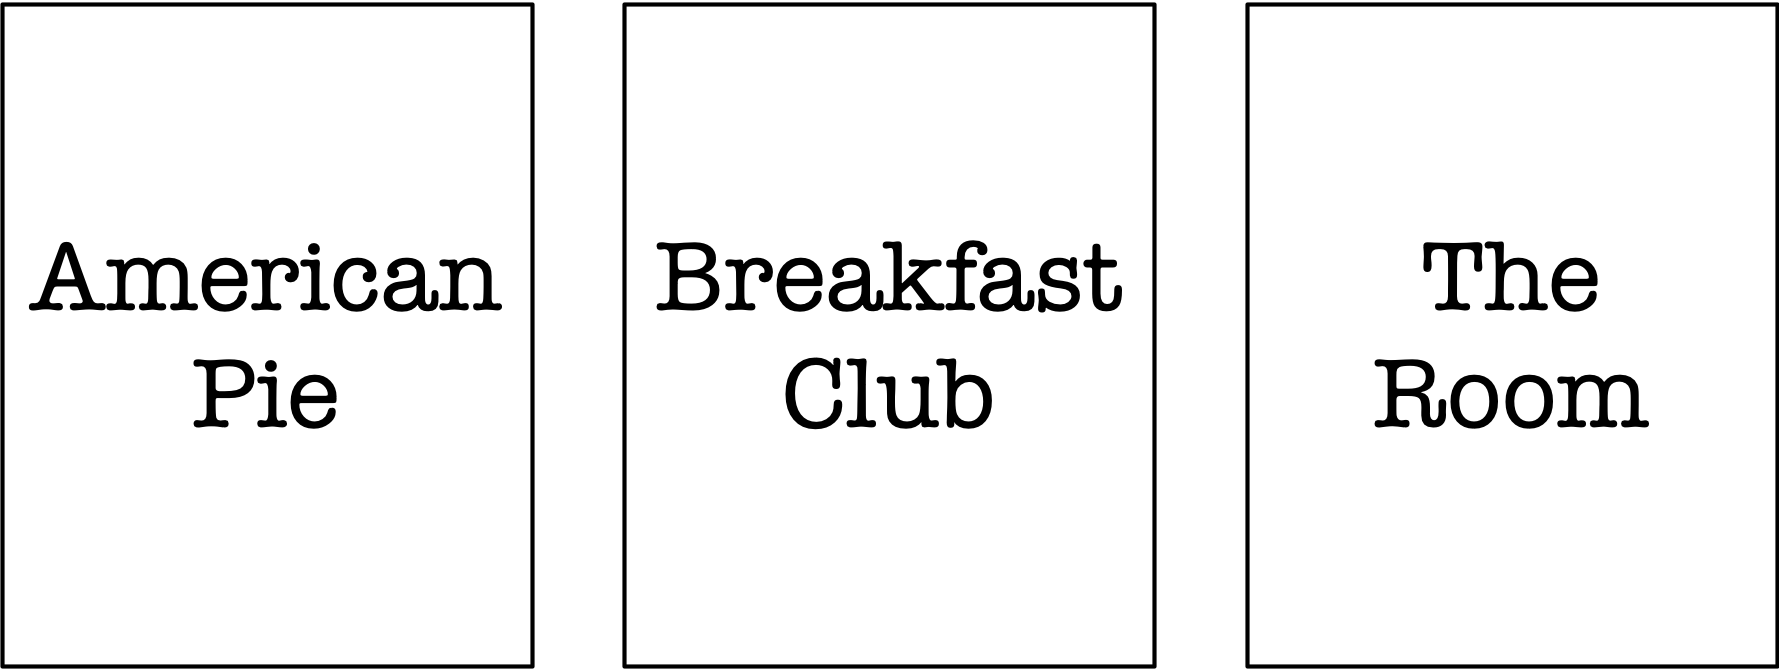
\includegraphics[width=\linewidth]{images/set_movies.png}
  \caption{Elements of set A.}
  \label{fig:marginfig}
\end{marginfigure}

A thing can be anything: name, object, idea. It's a very abstract notion. For example, I can define a set of movies I have seen: American Pie, Breakfast Club, The Room. Yes, I have only seen those three movies in my entire life. I am busy writing texts about set theory.

Actually, I've watched The Room five times. Does this affect the set? No, because it doesn't change the notion of "what movies I have watched". This obvious idea is an integral property of sets: they contain only unique objects.

\marginnote{Nothing stops us from defining a set of movie viewings, though. In that case, each element would be a particular instance of a "movie watching event", and, in my sad case, would contain 7 elements.}


If an object \(o\) is in set \(A\), we say \(o\) is a member of \(A\). To express this fact easily, mathematicians use the following notation: \(o \in A\).

So, if \(A = \textrm{Movies I've watched}\) and \(o = \textrm{The Room}\), then \(o \in A\). But if \(b = \textrm{Avengers}\),  then \(b \notin A\). Now you can generate infinitely many "nerdy" T-shirts with prints like \(\textrm{joy} \in \textrm{mylife}\) or \(\textrm{party} \in \textrm{dahouse}\).

If we were to look inside set \(A\), it might look like this:

\begin{equation}
\{s, m, o\}
\end{equation}

Sets don't have the notion of order, so it doesn't matter how you mention its members as long as you mention them all. So, all these:

\begin{itemize}
\item \(\{s, m, o\}\)
\item \(\{s, o, m\}\)
\item \(\{m, s, o\}\)
\item etc.
\end{itemize}

describe the same set \(A\).

We are lucky: set \(A\) is finite and quite small. But sets can be infinite, and it would be impossible to write down all of its members. There are ways to describe such sets nevertheless. For example, the set of all natural numbers from \(1\) to \(n\) can be described like so:

\begin{equation}
\{1, 2, 3, 4, ... n\}
\end{equation}

Here we rely on reader's common sense and assume he or she can rightfully deduce what is meant by the ellipsis (\texttt{...}). Notations like this are very common in math, and while it isn't awfully strict, the idea is to be as unambiguous as possible. For example, when describing a set of odd natural numbers from \(1\) to \(n\), this would be bad:

\begin{equation}
\{1, 3, ... n\}
\end{equation}

simply because the sample isn't long enough to make a single assumption.

Another example of a set that exists in math is the set of Boolean values:

\begin{equation}
\mathscr{B} = \{T, F\}
\end{equation}

\(T\) and \(F\) stand for \emph{True} and \emph{False}. Certain tests (or, in other words, questions) that can be answered with "yes" and "no", produce values of said set. So, we can say that

\begin{equation}
(x > y) \in \mathscr{B}, \textrm{where }  x \in \mathbb{N} \textrm{ and } y \in \mathbb{N}
\end{equation}

In other words, the answer to the question "is \(x\) greater than \(y\)" is a member of set \(\mathscr{B}\), as long as \(x\) and \(y\) are members of \(\mathbb{N}\) (i.e. natural numbers).

Math in infinitely composable. Most programming languages can only dream of the level of composability and flexibility mathematicians enjoy. While not immediately useful, we could compose the following statements about sets:

\begin{equation}
((x + y) \in \mathbb{N}) \in \mathscr{B}, \textrm{where }  x, y \in \mathbb{N}
\end{equation}

Here we said "when \(x\) and \(y\) are members of \(\mathbb{N}\), then the answer to the question 'is \(x + y\) a member of \(\mathbb{N}\)' is a member of \(\mathscr{B}\)."

Many groups in mathematics are sets: numbers of different types (natural, irrational, complex, etc.), notions of different types (e.g. Boolean), solutions to particular problems (e.g. graphs that satisfy a certain property). But describing groups of elements is just the tip of the iceberg. Set theory, with its axioms and definitions, can play a role of a foundational area of math, from which many other areas can be derived.

In this course and the book we're not going to talk about how set theory (and category theory) can "generate" a large portion of the whole math. But these topics are among the most fascinating frontiers of modern mathematics.

\section{Empty set}
\label{sec:org48e7535}

Mathematicians love zero. Ever since its inception around 1770 BC, zero is an important part of mathematical models. The notion of "nothingness", which zero reflects in the context of counting, is present in all areas. In the context of sets, nothingness is an \emph{empty set}.

\begin{equation}
\varnothing = \{\}
\end{equation}

Why would we need empty sets? Well, sometimes we want to describe a notion of having no objects under a certain description. For example, since I only watched 3 movies in my life, and all of them were American, I can describe:

\begin{equation}
\varnothing = \textrm{the set of all non-American movies I've watched}.
\end{equation}

A more mathematical example would be something like this:

\begin{equation}
\varnothing = \{x | x \in \mathbb{N} \textrm{ and } x < 0\}
\end{equation}

which says that the set of natural numbers smaller than zero is an empty set. It's a formal way to say that there are no natural numbers less than zero.

Note the use of vertical line \textbf{\texttt{|}}, it is a shorter way to say "where".

\section{Subset, superset}
\label{sec:org3f004ec}

When all members of set \(A\) are present in another set \(B\), then \(A\) is a \textbf{subset} of \(B\). Let's say set \(B\) is the set of all movies ever produced. Then \(A\) (movies I've watched) is clearly a subset of \(B\). This notion is expressed like so:

\begin{equation}
A \subseteq B
\end{equation}

To look at things from the other end, \(B\) is a \textbf{superset} of \(A\):

\begin{equation}
B \supseteq A
\end{equation}

\begin{marginfigure}
  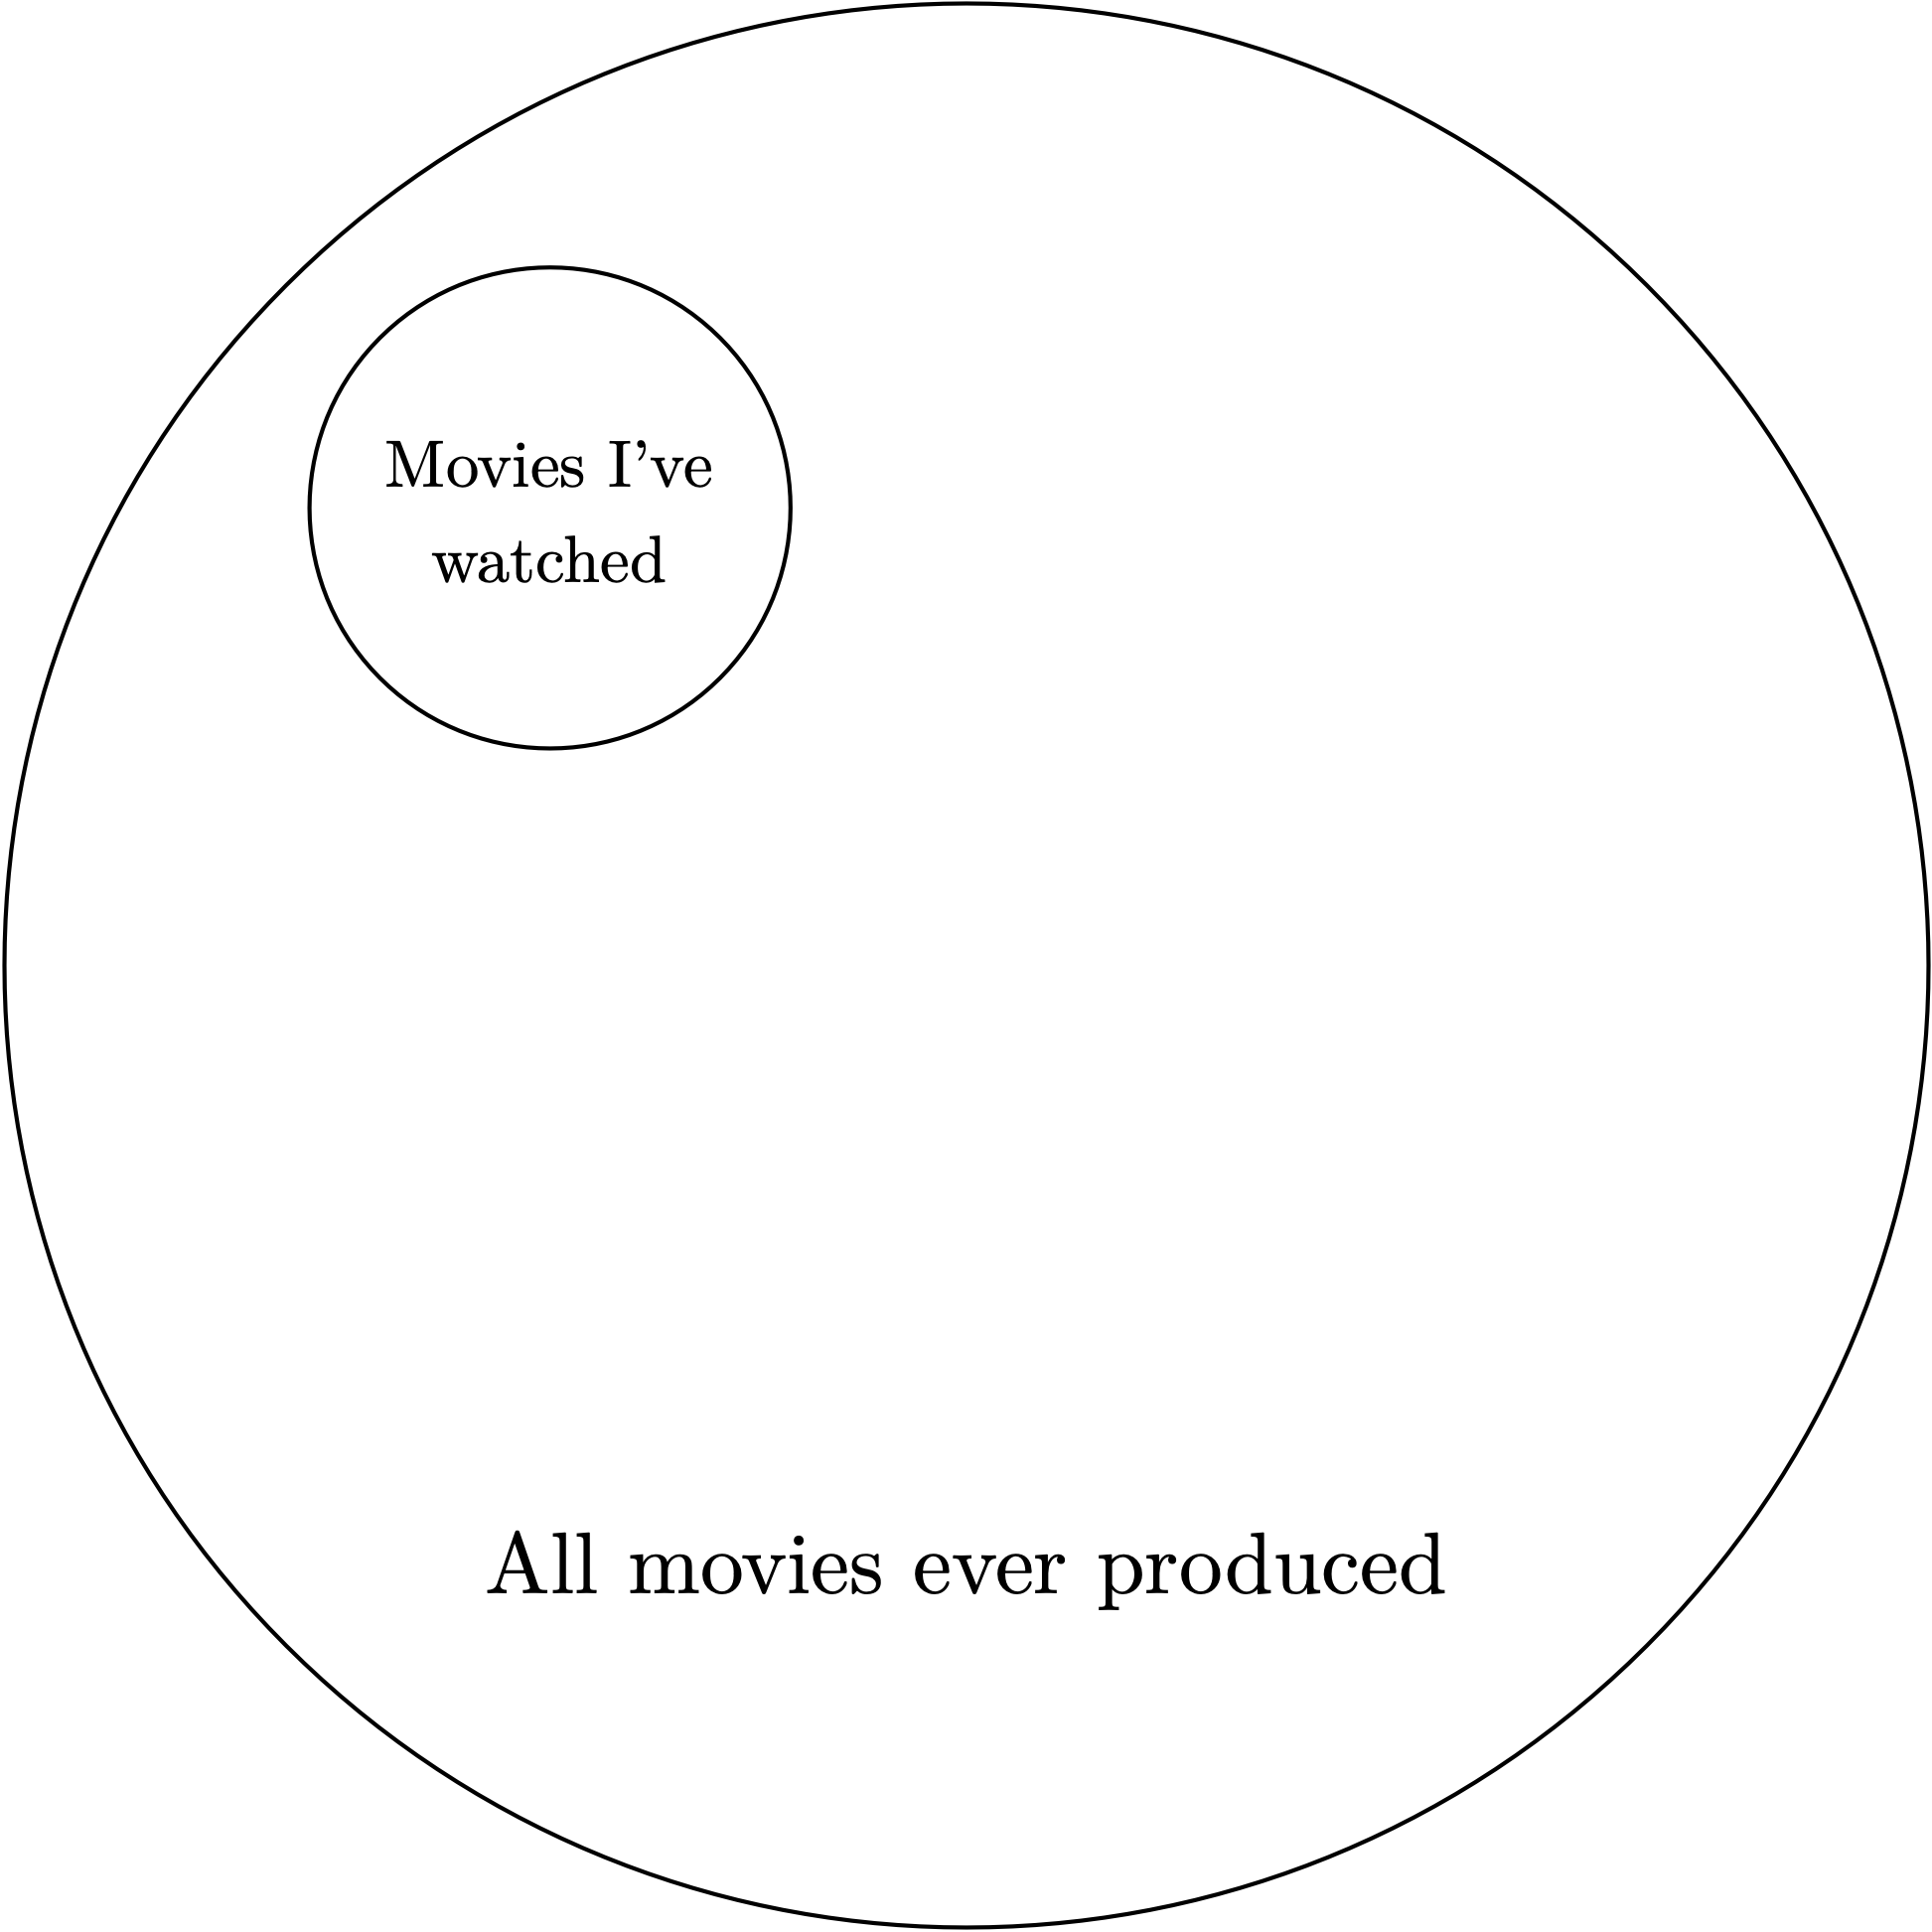
\includegraphics[width=\linewidth]{images/subset.png}
  \caption{A set and its subset.}
  \label{fig:marginfig}
\end{marginfigure}


You know what else is a subset of \(B\)? An empty set!

\begin{equation}
\varnothing \subseteq B
\end{equation}

This either sounds absolutely natural to you or extremely weird. It makes perfect sense to a mathematician, because it's easy to argue: \emph{all} members of \(\varnothing\) are present in \(B\), all zero of them.

It gets weirder. As per our definition, if all members of a set are also present in another set, then the one is a subset of the other. This means any set is a subset of itself.

\begin{equation}
\displaylines{
A \subseteq A \\
B \subseteq B \\
Z \subseteq Z
}
\end{equation}

By extension, if two sets are the same, then either of them is a subset of the other.

\begin{equation}
\textrm{if } A \subseteq B \textrm{ and } B \subseteq A \textrm{ then } A = B
\end{equation}

When we look at a statement \(A \subseteq B\), we often need to know whether \(A = B\) or not. To distinguish between the two cases, mathematicians use a special notion of a \textbf{proper subset}.

If \(A \subseteq B\), but \(A \neq B\), then \(A\) is a proper subset of \(B\).

\begin{equation}
A \subset B
\end{equation}

Since I haven't watched all the movies ever produced, I can say that \(A\) is a proper subset of \(B\). So, a set is a subset of itself, but is never a proper subset of itself.
\section{Cardinality}
\label{sec:org8a30fe7}

Before we start to talk about sizes and products, let's first introduce a new notion:  \textbf{\textbf{sequence}}. A sequence is simply a series of elements. Unlike sets, sequences have order and may contain duplicate values. In this sense sequences are more down to earth, practical collections.

Sequences are written with round brackets. For example, a sequence of prime numbers in ascending order is:

\begin{equation}
(2, 3, 5, 7, 11, ...)
\end{equation}

Note that it is an infinite sequence. An example of a finite sequence is a sequence of natural even numbers smaller than 10:

\begin{equation}
(1, 2, 3, 4, 5, 6, 7, 8, 9)
\end{equation}

\noindent\rule{\textwidth}{0.5pt}

If \(A\) is a finite set (that is, \(A\) is not infinite, and we can count how many elements there are in it), we use \(|A|\) to denote the number of elements of \(A\). This is the \textbf{\textbf{cardinality}}. For example:

\begin{equation}
\displaylines{
|\{4, 8, 15, 16, 23, 42\}| = 6, \\
|\varnothing| = 0, \\
|\{\{a, e\}\}| = 1.
}
\end{equation}

Note the last example: it defines a set which contains one set, thus its cardinality is 1. The number of elements of the internal set is irrelevant. Programmers find this obvious, as it reminds them of nested data structures like arrays of arrays.

Knowing about sets, subsets and cardinalities, let's look at a statement and prove it.

\textbf{Statement 1}: \emph{If \(A\) is a finite set of \(m\) elements, then there are \(2^{m}\) subsets of \(A\).}

\textbf{Proof}: Suppose \(A = \{a_{1}, a_{2}, ..., a_{m}\}\) and \(\mathscr{P}A\) is the set of all subsets of \(A\). Then we can divide \(\mathscr{P}A\) into \(2=2^{1}\) collections: subsets of \(A\) which contain \(a_{1}\) and those which don't. Considering the next element \(a_{2}\), we get 4=2\(^{\text{2}}\) collections:

\begin{enumerate}
\item One which contains both \(a_{1}\) and \(a_{2}\),
\item one which contains \(a_{1}\), but not \(a_{2}\),
\item one which contains \(a_{2}\), but not \(a_{1}\),
\item one which contains neither \(a_{1}\) nor \(a_{2}\).
\end{enumerate}

Continuing this way, we see that there are \(2^{m}\) subsets of \(A\), each subset is determined by the fact of whether or not each \(a_{j}\) is included, as \(j\) goes from \(1\) to \(m\).

This sort of counting by inclusion / exclusion is a popular technique in math and especially in computer science. One can visualize such proof for a particular case by drawing a "binary decision tree".

Consider set \(A = \{a_{1}, a_{2}, a_{3}\}\). The proof states that there are \(2^{3} = 8\) subsets of \(A\). Do describe each imaginable set we need to determine whether each element is in it or not. Starting from \(a_{1}\), we need to answer "yes" or "no", and proceed to ask the same question for \(a_{2}\) and then for \(a_{3}\).


\begin{figure*}[htbp]
\centering
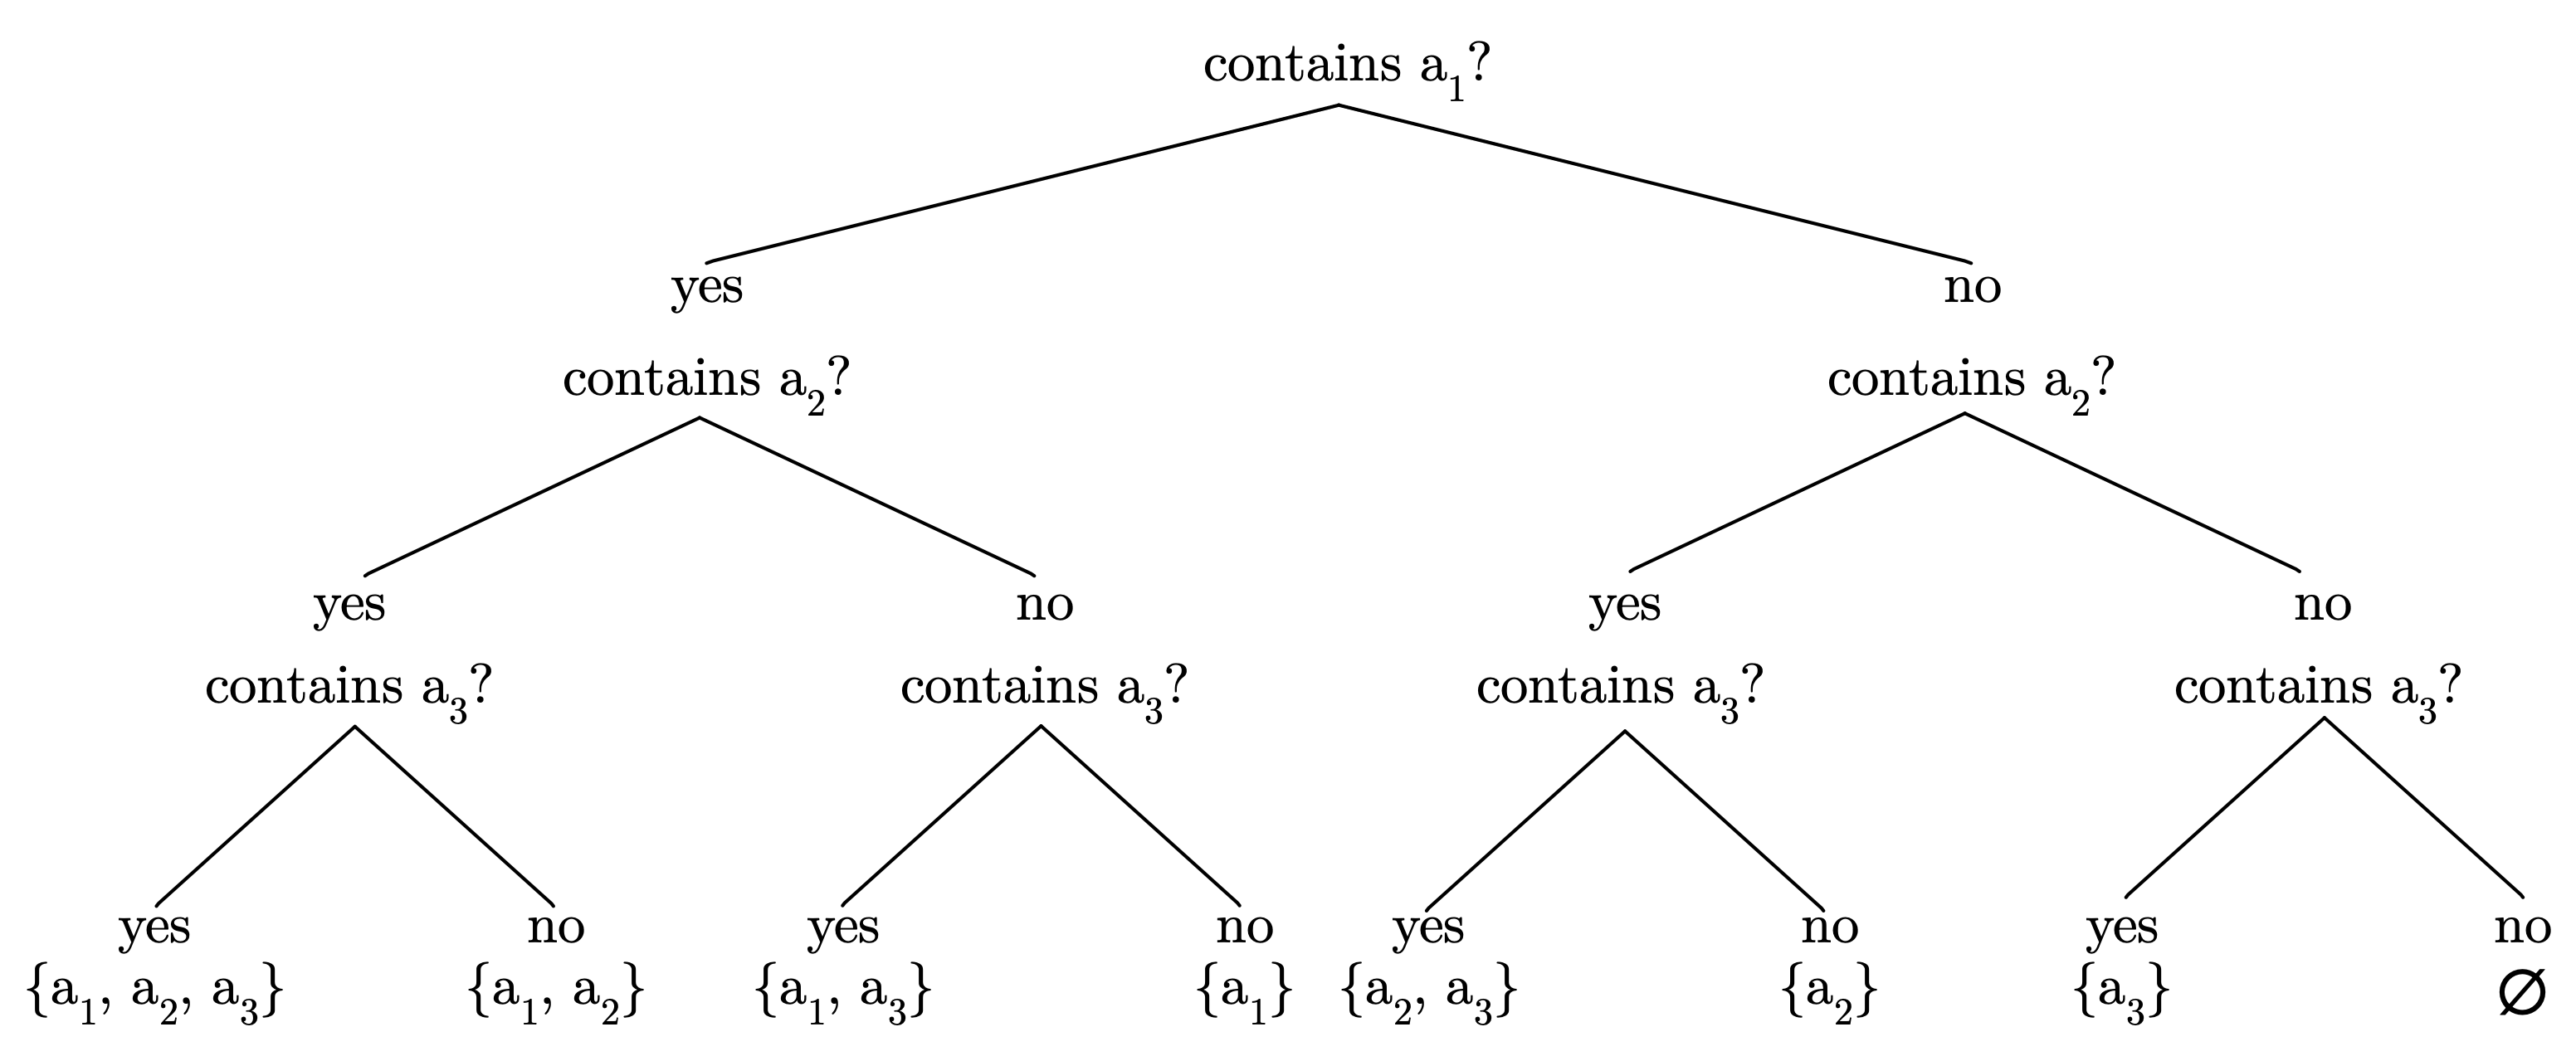
\includegraphics[width=.9\linewidth]{./images/powerset_binary_decision_tree.png}
\caption{\label{fig:orge2eb83a}
Binary decision tree for 8 subsets of \{a_{1}, a_{2}, a_{3}\}}
\end{figure*}

\section{Cartesian product}
\label{sec:org9fefb3f}

Given two sets \(A\) and \(B\), we are often interested in all ordered pairs of their elements. For example, if \(A = \{a, b\}\) and \(B = \{1, 2\}\), the ordered pairs are as follows:

\begin{equation}
\displaylines{
(a, 1)\\
(a, 2)\\
(b, 1)\\
(b, 2)\\
}
\end{equation}

The set of all such pairs is called the \textbf{Cartesian product} of \(A\) and \(B\). The name comes from the French mathematician René Descartes.

\begin{marginfigure}
  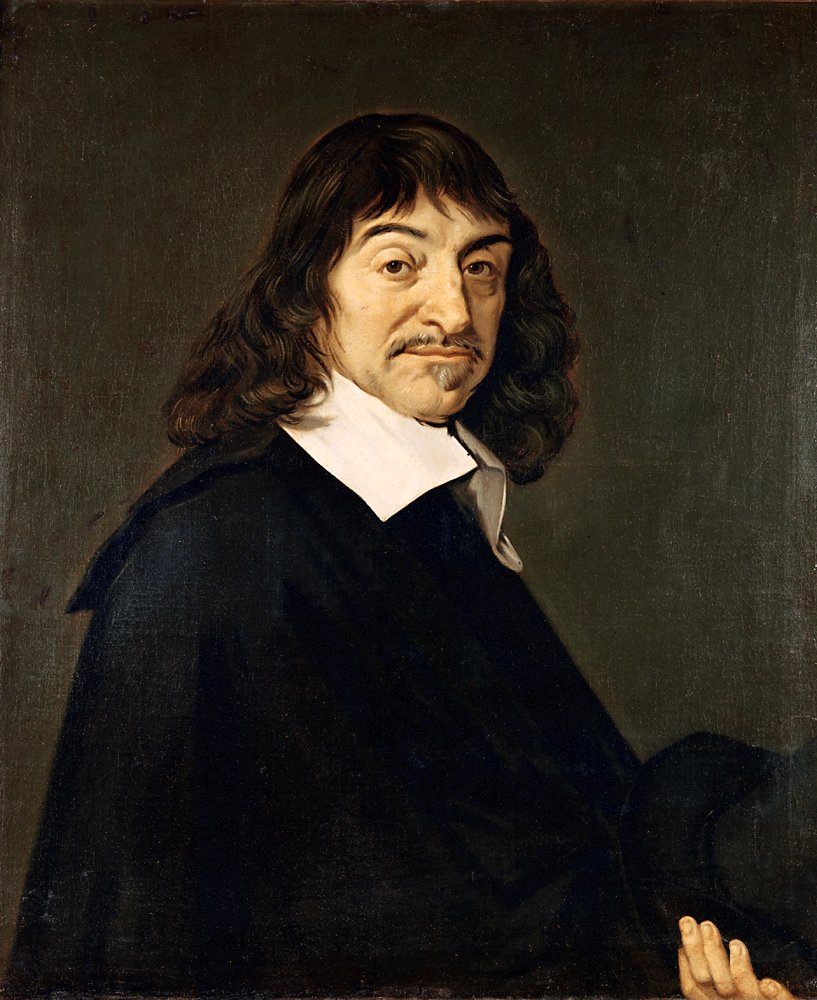
\includegraphics[width=\linewidth]{images/Frans_Hals_-_Portret_van_Rene_Descartes.jpg}
  \caption{Frans Hals, Portret van René Descartes}
  \label{fig:marginfig}
\end{marginfigure}

Formally, Cartesian product can be described like this:

\begin{equation}
A \times B = \{(a,b) | a \in A, b \in B\}
\end{equation}

Descartes saw that the number plane \(x, y\) could be represented as a product of two sets of real numbers.

\begin{equation}
\mathbb{R} \times \mathbb{R} = \{(x, y) | x \in \mathbb{R}, y \in \mathbb{R}\}
\end{equation}

\begin{figure}[htbp]
\centering
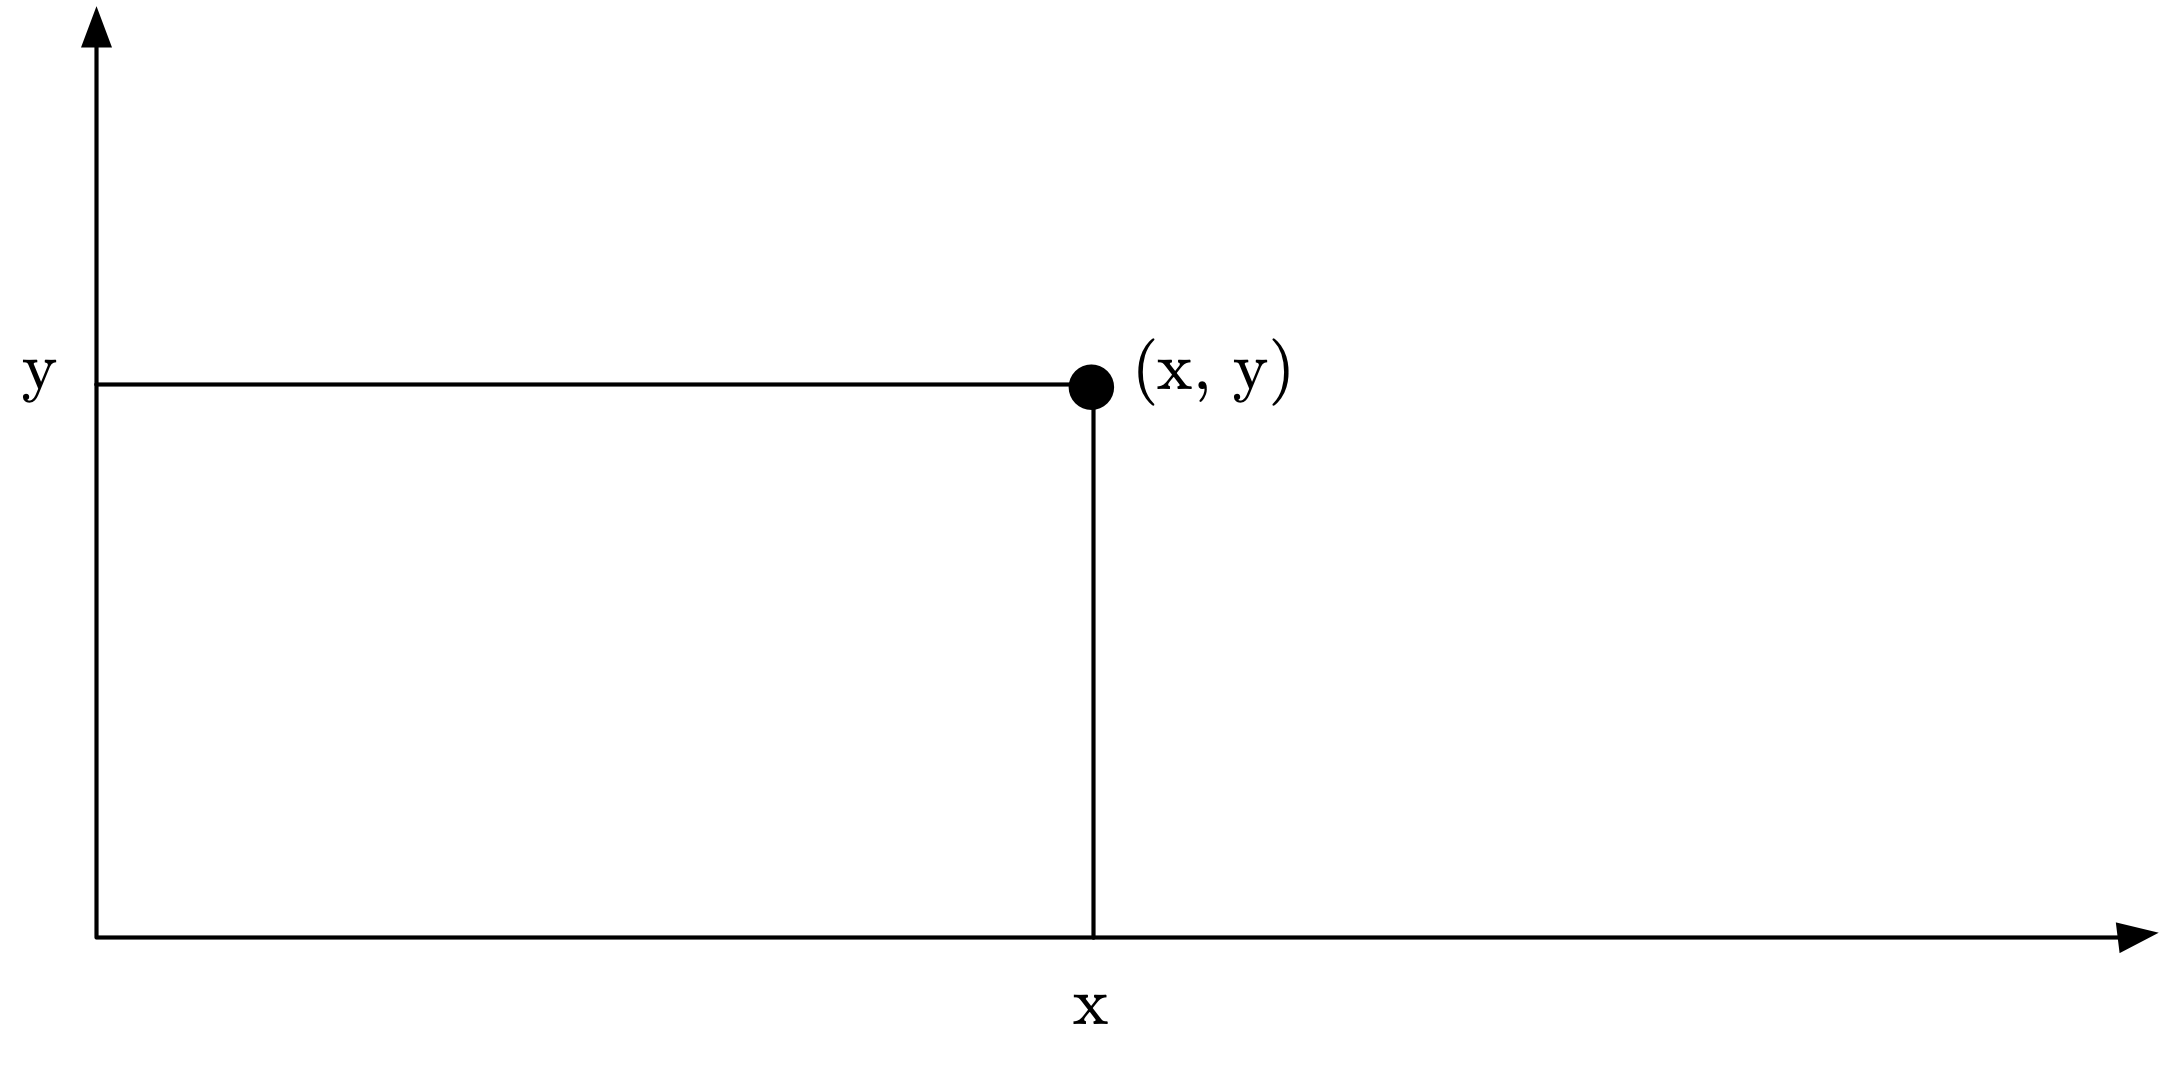
\includegraphics[width=.9\linewidth]{./images/xy_plane.png}
\caption{\label{fig:orge2eb83a}
Each point on x, y plane is in the Cartesian product of 2 sets of real numbers.}
\end{figure}

\section{Union}
\label{sec:org675e6b5}

Sets on their own are a bit boring, frozen things. Interesting results can be observed when we consider interactions between sets. At the same time, these interactions can be viewed as frozen things themselves, not actions or processes.

This happens often in math: the same idea can be viewed as either an action or a thing. Even functions, seemingly action-able, moving notions, can (and will) be defined as mere static constructs. It's interesting to ponder about these things, draw analogies to physics and time.

Regardless, let's quickly overview three main sorts of interactions. Chances are they are already very familiar to you, especially if you've done any SQL.

\textbf{\textbf{Union}} of a collection of sets is the set of all elements of the collection.

Given two sets \(A\) and \(B\), union is defined as:

\begin{equation}
A \cup B = \{ x | x \in A \textrm{ or } x \in B \}
\end{equation}

This reads as:

\begin{quote}
Union of \(A\) and \(B\) is a set of elements \(x\), where \(x\) belongs to \(A\) or x belongs to \(B\).
\end{quote}

For example, if \(A = \{1, 2, 3\}\), and \(B = \{3, 4, 5\}\), then:

\begin{equation}
A \cup B = \{1, 2, 3, 4, 5\}
\end{equation}

Note that even though each set contains 3 elements, the resulting union contains 5 elements only. Since union is a set, all rules and properties regarding sets still apply, so it cannot contain element \(3\) twice.

It is sometimes necessary to keep duplicates somehow, without violating the rules of sets. One way is "tag" each element in both sets by generating a Cartesian product of each set.

\begin{equation}
\displaylines{
A \times \{t_{A} \} = \{(1, t_{A}), (2, t_{A}), (3, t_{A}) \} \\
B \times \{t_{B} \} = \{(3, t_{B}), (4, t_{B}), (5, t_{B}) \}
}
\end{equation}

So now instead of each number we deal with a sequence of two elements: the original number and a tag which refers to the original set. We use the term \emph{n-tuple} for a sequence of length \(n\). Thus, here we deal with sets of \emph{2-tuples}.

Since all tuples are unique, the resulting union set contains 6 distinct elements:

\begin{equation}
\displaylines{
A \times \{t_{A} \} \cup B \times \{t_{B} \} = \\
\{(1, t_{A}), (2, t_{A}), (3, t_{A}), (3, t_{B}), (4, t_{B}), (5, t_{B}) \}
}
\end{equation}

Every time we learn about a new approach or an idea, your inner mathematician should aspire to generalize. We've already generalized the notion of union by providing a formal mathematical definition. Let us now define this so-called \textbf{\textbf{disjoint union}} \(\sum A_{i}\) to be:

\begin{equation}
\bigcup_{1 \leq i \leq n} A_{i} \times \{i\} = \{(x, i) | x \in A_{i} \textrm{ and } 1 \leq i \leq n\}
\end{equation}

It might seem like the notation is getting more and more complicated, but it's only a combination of existing notions and symbols, nothing new. The big U is a generalization of unions, here it is limited to all sets \(A_{i} \times \{i\}\) where \(i\) goes from 1 to some \(n\). You can think of \(i\) as a variable or a parameter. We see it is then used to define different sets (e.g. \(A_{1}\), \(A_{2}\), etc) and corresponding tagging sets \(\{1\}\), \(\{2\}\), etc. Then, on the right-hand side of the equation there's a set of many 2-tuples, each containing an element from \(A_{i}\) and a tagging number \(i\).

To easily differentiate between regular unions and disjoint unions, we use two different symbols: \(\cup\) for union, \(+\) for disjoint union. Thus:

\begin{equation}
\bigcup_{1 \leq i \leq n} A_{i} \times \{i\} = A_{1} + ... + A_{n}.
\end{equation}

\noindent\rule{\textwidth}{0.5pt}

Even if you haven't heard of set union, you've definitely seen Venn diagrams. They illustrate union, intersection and complement quite nicely.

\url{https://s3.amazonaws.com/thinkific/file\_uploads/146581/images/8cf/e18/857/British\_Isles\_Venn\_Diagram-en.svg.png}

Contrary to popular belief, Venn diagrams aren't suitable representations of \texttt{SQL JOIN}. You'll see why later.

When working with databases using SQL, union operation is a direct equivalent of union from set theory. The following example returns all usernames of both customers and managers:

\begin{verbatim}
SELECT username FROM users
UNION
SELECT username FROM managers;
\end{verbatim}

This regular \texttt{UNION} operation behaves like set union in regards to duplicates. Thus, if both tables contain identical usernames, only one instance would end up in the union. An alternative SQL operator \texttt{UNION ALL} allows duplicates. The resulting collection of records is not necessarily a set, since it main contain identical records.

It is tempting to see SQL as set theory applied to databases, but it would be wrong to think this way. SQL can be considered a domain specific language for a particular application of relational algebra, which \emph{incorporates} certain areas of set theory. In general, one can say that set theory and SQL \emph{intersect}.

\section{Intersection}
\label{sec:orgefe83a0}

\textbf{\textbf{Intersection}} of two sets \(A\) and \(B\) is the set containing all elements of \(A\) that also belong to \(B\) (or vice versa). In other words, it's a set of common elements.

\begin{equation}
A \cap B = \{ x : x \in A \textrm{ and } x \in B \}
\end{equation}

This reads as:

\begin{quote}
Intersection of \(A\) and \(B\) is the set of elements \(x\), where \(x\) belongs to \(A\) and x belongs to \(B\).
\end{quote}

For example, if \(A = \{1, 2, 3\}\), and \(B = \{3, 4, 5\}\), then 3 is the only element present in both sets:

\begin{equation}
A \cap B = \{3\}
\end{equation}

\emph{Sidenote: I quickly remembered which symbol -- \(\cup\) and \(\cap\) -- means which operation by noticing that \(\cup\) looks like letter U, so it means union. I've had a similar moment when learning Boolean algebra and logic, where \(\wedge\) means AND and looks like \(A\) without the horizontal bar.}

SQL has \texttt{INTERSECT}:

\begin{verbatim}
SELECT username FROM customers
INTERSECT
SELECT username FROM managers;
\end{verbatim}

Naturally, duplicates aren't an issue for intersection, because by definition one pair of elements results in one element, and not two. If there are two elements in one set, and one same element in the other set, the result is still one common element in the intersection.

A Venn diagram for intersection is often used to show commonality. For example, coming back to sets of favorite movies, we can compare your favorite movies and mine and see if there are any movies we both love. If no such movies exist, then our sets are \textbf{\textbf{disjoint}}. Formally, two sets are disjoint if their intersection is an empty set:

\begin{equation}
A \cap B = \varnothing
\end{equation}

A mathematician in love may describe the perfectness of their partner by saying that the partner's qualities and bad qualities are disjoint sets. The partner would definitely accept this as a complement (sic)\ldots{}

\section{Complement (difference)}
\label{sec:org6d0ccb7}

\textbf{\textbf{Complement}} of set \(A\) is a set of elements not in \(A\). In other words, it's the opposite of \(A\).

\begin{equation}
A^{C} = \{x : x \notin A \}
\end{equation}

The notion of complement (or difference) requires an implicit assumption: what other elements are we talking about? Say, the complement of all positive numbers is negative numbers, and zero, and dogs, and Korean words, and\ldots{} all possible elements that aren't positive numbers? Thinking this way quickly reduces the conversation to either absurdity or to Russell's paradox. This is why the complement assumes some larger set in which \(A\) exists. This larger set should be obvious from the context, or should be specified explicitly somewhere. For instance, when talking about movies, the complement of the set of my favorite movies is obviously all other movies that aren't my favorite.

The term \textbf{universe} is used for a collection of entities one wishes to consider. For the example of movies, the universe is probably "all movies ever produced".

\noindent\rule{\textwidth}{0.5pt}

It's sometimes useful to consider the complement of a set with respect to some other well-defined set. This is often called \textbf{set difference} and is denoted as \(A - B\). Formally:

\begin{equation}
A - B = \{x | x \in A \textrm{ but } x \notin B\}
\end{equation}

SQL operator \texttt{EXCEPT} is similar to this idea.

\begin{verbatim}
SELECT username FROM users
EXCEPT
SELECT username FROM managers;
\end{verbatim}

This query would return all users who aren't managers. In set theory, we'd write it this way:

\begin{equation}
\textrm{Users} - \textrm{Managers}
\end{equation}

Or, with implicit universe:

\begin{equation}
\textrm{Managers}^{C}
\end{equation}

with an assumption that we're talking about users in general.

\section{Relational algebra}
\label{sec:org0a19f1b}

If you worked with SQL in different databases, you might've noticed slight differences or even large, annoying discrepancies. The reason is that SQL isn't a formal, strict language, but rather an approach based on a general formal language called Relational algebra. Developers of different databases design their own versions of SQL and implement and modify its features at their discretion.

Relational algebra was created by Edgar F. Codd in 1960s-1970s, who worked at IBM at the time. Codd proposed this formal language as a basis for database querying.

The good news is that knowing set theory and relational algebra reduces potential SQL-related problems to basically documentation lookup. If you know how unions work, what's the idea behind a Cartesian product and what are expressions of relational algebra, then it comes down to finding the correct SQL syntax to solve the problem at hand.

We will finish up the section on set theory with a short overview of different aspects of relational algebra and their relation to SQL.

\begin{enumerate}
\item Relation
\label{sec:org05f18b3}

\textbf{\textbf{Relation}} is essentially a table, with columns (called "attributes") and rows. For example, a relation \texttt{User} may be used to describe users in a web service.

\begin{verbatim}
User(id, username, firstName, lastName, email)
\end{verbatim}

\begin{center}
\begin{tabular}{rllll}
id & username & firstName & lastName & email\\
\hline
1 & jenn & Jenn & Clarkson & jnc@hotmail.com\\
2 & pax & Paxi & Romanov & paxro@aol.com\\
91 & thankso & Barack & Liu & bl@wh.gov\\
\end{tabular}
\end{center}

For demonstrating purposes, let's define another table:

\begin{verbatim}
Manager(id, department, level)
\end{verbatim}

\begin{center}
\begin{tabular}{rlr}
id & department & level\\
\hline
1 & engineering & 3\\
2 & medicine & 2\\
91 & mathematics & 3\\
\end{tabular}
\end{center}

The name of a relation can play a role of the simplest query:

\begin{verbatim}
User
\end{verbatim}

which returns the whole table.

\item Projection
\label{sec:org4a320aa}

A \textbf{\textbf{projection}} is an operation of extracting records with specific columns (attributes). It is denoted by Greek letter \(\Pi\) (uppercase pi), with a list of columns as subscript, followed by relation's name.

For example, here we extract a sub-relation of User with ids and emails only:

\begin{equation}
\Pi_{\textrm{id, email}} \textrm{ User}
\end{equation}

\begin{center}
\begin{tabular}{rl}
id & email\\
\hline
1 & jnc@hotmail.com\\
2 & paxro@aol.com\\
91 & bl@wh.gov\\
\end{tabular}
\end{center}

\item Select
\label{sec:orgde51a66}

A \textbf{\textbf{selection}} is an operation of filtering records by values. It is denoted by Greek letter \(\sigma\) (sigma) with a condition, followed by relation's name.

For example, here we get managers with level higher than 2:

\begin{equation}
\sigma_{\textrm{level} > 2} \textrm{ Manager}
\end{equation}

\begin{center}
\begin{tabular}{rlr}
id & department & level\\
\hline
1 & engineering & 3\\
2 & medicine & 2\\
91 & mathematics & 3\\
\end{tabular}
\end{center}

\item Operating on expressions
\label{sec:orgdcada5c}

Select and project operators work on any expression, not only on whole relations. This means we can combine them arbitrarily. For example, we can select (essentially, filter) first, and then extract certain columns.

\begin{equation}
\Pi_{\textrm{id, level}} (\sigma_{\textrm{level} > 2} \textrm{ Manager})
\end{equation}

The result is a newly constructed relation consisting of only two columns, which, in turn, can be used for other operations:

\begin{center}
\begin{tabular}{rr}
id & level\\
\hline
1 & 3\\
91 & 3\\
\end{tabular}
\end{center}

\item Cross product (cartesian product)
\label{sec:orgcb1409f}

Recall the idea behind Cartesian product in set theory: given two sets \(A = \{a, b\}\) and \(B = \{1, 2\}\), the \textbf{Cartesian product} is a set of pairs of all combinations of elements:

\begin{equation}
\displaylines{
(a, 1)\\
(a, 2)\\
(b, 1)\\
(b, 2)\\
}
\end{equation}

Much of the power of relational algebra comes from applying this idea to relations. It is also often called \textbf{cross product}.

Here's the cross-product of \texttt{User} and \texttt{Manager}:

\begin{equation}
\textrm{User} \times \textrm{Manager}
\end{equation}

\begin{center}
\begin{tabular}{rllllrlr}
User.id & username & firstName & lastName & email & Manager.id & department & level\\
\hline
1 & jenn & Jenn & Clarkson & jnc@hotmail.com & 1 & engineering & 3\\
1 & jenn & Jenn & Clarkson & jnc@hotmail.com & 2 & medicine & 2\\
1 & jenn & Jenn & Clarkson & jnc@hotmail.com & 91 & mathematics & 3\\
2 & pax & Paxi & Romanov & paxro@aol.com & 1 & engineering & 3\\
2 & pax & Paxi & Romanov & paxro@aol.com & 2 & medicine & 2\\
2 & pax & Paxi & Romanov & paxro@aol.com & 91 & mathematics & 3\\
91 & thankso & Barack & Liu & bl@wh.gov & 1 & engineering & 3\\
91 & thankso & Barack & Liu & bl@wh.gov & 2 & medicine & 2\\
91 & thankso & Barack & Liu & bl@wh.gov & 91 & mathematics & 3\\
\end{tabular}
\end{center}

Since both relations contain a column named \texttt{id}, the resulting relation contains two distinct columns with tagged names \texttt{User.id} and \texttt{Manager.id}. This is similar to the way we "tagged" items in set union.

This might not seem too useful: we just combined all records, and many of the new rows don't make sense. Cross-product is rarely useful as is. Instead, the goal is often to generate raw data for the operations. For example, with this long table at hand, we can first eliminate the nonsense rows by applying select:

\begin{equation}
\sigma_{\textrm{User.id} = \textrm{Manager.id}} (\textrm{User} \times \textrm{Manager})
\end{equation}


\begin{center}
\begin{tabular}{rllllrlr}
User.id & username & firstName & lastName & email & Manager.id & department & level\\
\hline
1 & jenn & Jenn & Clarkson & jnc@hotmail.com & 1 & engineering & 3\\
2 & pax & Paxi & Romanov & paxro@aol.com & 2 & medicine & 2\\
91 & thankso & Barack & Liu & bl@wh.gov & 91 & mathematics & 3\\
\end{tabular}
\end{center}

Assuming user ids in the system are used to identify managers as well, we now have a sensible relation of managers with their complete user info intact.

Now we can filter managers by level and get rid of unneeded columns:


\begin{equation}
\Pi_{\textrm{User.id, email, department}}
\big(
\sigma_{\textrm{User.id} = \textrm{Manager.id}, \textrm{level} > 2} (\textrm{User} \times \textrm{Manager})
\big)
\end{equation}

\begin{center}
\begin{tabular}{rll}
User.id & email & department\\
\hline
1 & jnc@hotmail.com & engineering\\
91 & bl@wh.gov & mathematics\\
\end{tabular}
\end{center}

\item Natural join
\label{sec:org1c50a49}

The process of performing a cross-product and then filtering out rows that "make sense" by comparing the attributes of the same name is common enough so that relational algebra has a special operator called \textbf{natural join}. It is denoted by \(\bowtie\) (bow tie). The result is a relation with matching rows and no "tagged" attributes:

\begin{equation}
\textrm{User} \bowtie \textrm{Manager}
\end{equation}

\begin{center}
\begin{tabular}{rlllllr}
id & username & firstName & lastName & email & department & level\\
\hline
1 & jenn & Jenn & Clarkson & jnc@hotmail.com & engineering & 3\\
2 & pax & Paxi & Romanov & paxro@aol.com & medicine & 2\\
91 & thankso & Barack & Liu & bl@wh.gov & mathematics & 3\\
\end{tabular}
\end{center}

As you see, natural join is basically a syntactic sugar on top of existing features of relational algebra.

\item Union, intersection, difference
\label{sec:org7c228cb}

Relational algebra includes three operators straight from set theory: union, intersection and difference. They work just like you might expect, although there are some caveats. We will not focus on these topics at the moment.
\end{enumerate}

\section{Relations and Functions}
\label{sec:org603c575}

In programming, we often deal with paired data:

\begin{itemize}
\item username — email
\item person — phone number
\item id — company
\end{itemize}

All cases can be considered as two sets, with a rule to connect their elements.

Given two sets \(A\) and \(B\), a \emph{map function} \(f\) from \(A\) to \(B\), denoted as

\begin{equation}
f: A \rightarrow B
\end{equation}

is an assignment  to each element \(a\) in \(A\) of a single element in \(B\).

We sometimes use a notation \(a \mapsto f(a)\) (note the different arrow) to indicate that \(a\) maps to some value via function \(f\). We call \(f(a)\) an \emph{image} of \(a\). Set \(A\) is called the \emph{domain} of \(f\), and \(B\) the \emph{codomain} of \(f\).

Notice how we talk about functions as static data, not as a process. In programming, we're used to functions being descriptions of processes, even though in most languages we can pass functions around as data. But consider this: how would you cache a function call? An obvious approach is to pre-compute some answers beforehand and store them in a table:

\begin{center}
\begin{tabular}{lr}
Argument & Return\\
\hline
"a" & 52321\\
"b" & 12321\\
"c & 81872\\
\ldots{} & \ldots{}\\
\end{tabular}
\end{center}

Theoretically, we could do this for all possible arguments, which would allow us to disregard all function's code and continue operating with a cache table exclusively. This means that any function (unless it deals with randomization) can be represented as static data. A mathematical notation of a function as a relation between two sets (essentially, a set of arguments and a set of return values) generalizes this idea.

A \textbf{binary relation} of two sets \(A\) and \(B\) is a subset of \(A \times B\). (Recall that \(A \times B\) is a set of all combinations of pairs of values of the two sets). Thus, a \emph{function} is a binary relation, having the property that for each element \(a \in A\) there is exactly one ordered pair in \(A \times B\) whose first component is \(a\).

There are three types of relations:

\textbf{1.} The function \(f: A \rightarrow B\) is \emph{one-to-one} (\textbf{injective}) if no two values of \(A\) result in the same value of \(B\). In other words, there's at most one incoming arrow for each element of \(B\).

Formally: for any two distinct elements \(a\) and \(a'\) in \(A\), we have \(f(a) \neq f(a')\).

\begin{figure}
  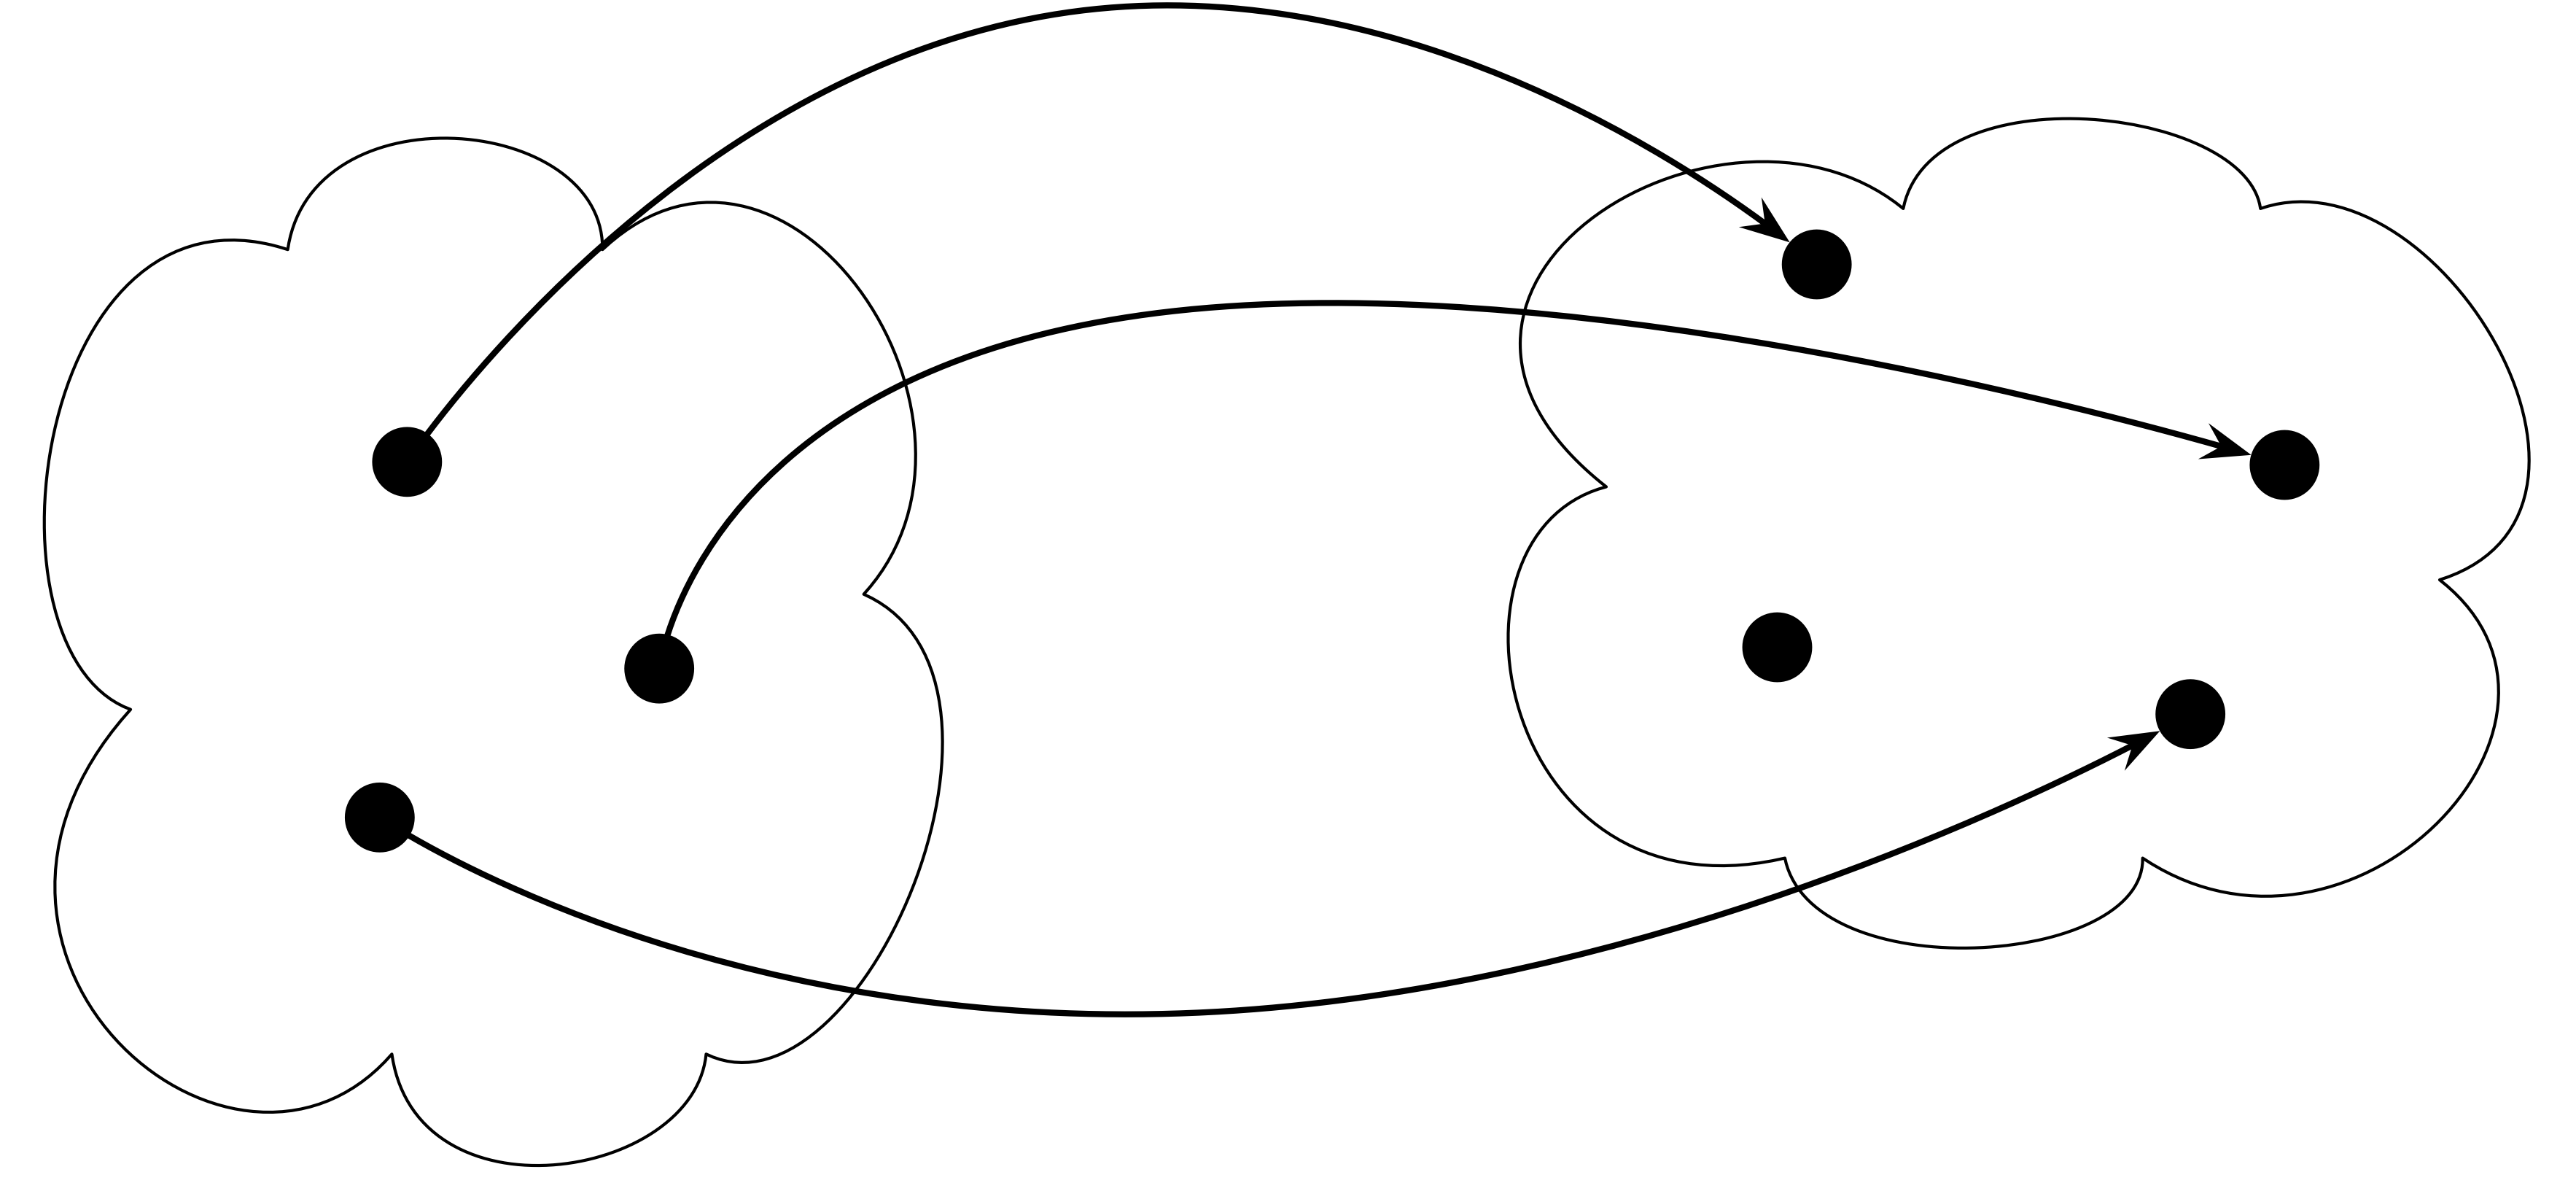
\includegraphics[width=.5\linewidth,right]{images/relations/injection.png}
  \caption{Injection.}
  \label{fig:injection}
\end{figure}

\textbf{2.} The function \(f: A \rightarrow B\) is \emph{onto} (\textbf{surjective}) if all elements of \(B\) are covered. In other words, no element of \(B\) is without at least one arrow.

Formally: for each element \(b \in B\), there exists an element \(a \in A\), such that \(f(a) = b\).

\begin{figure}
  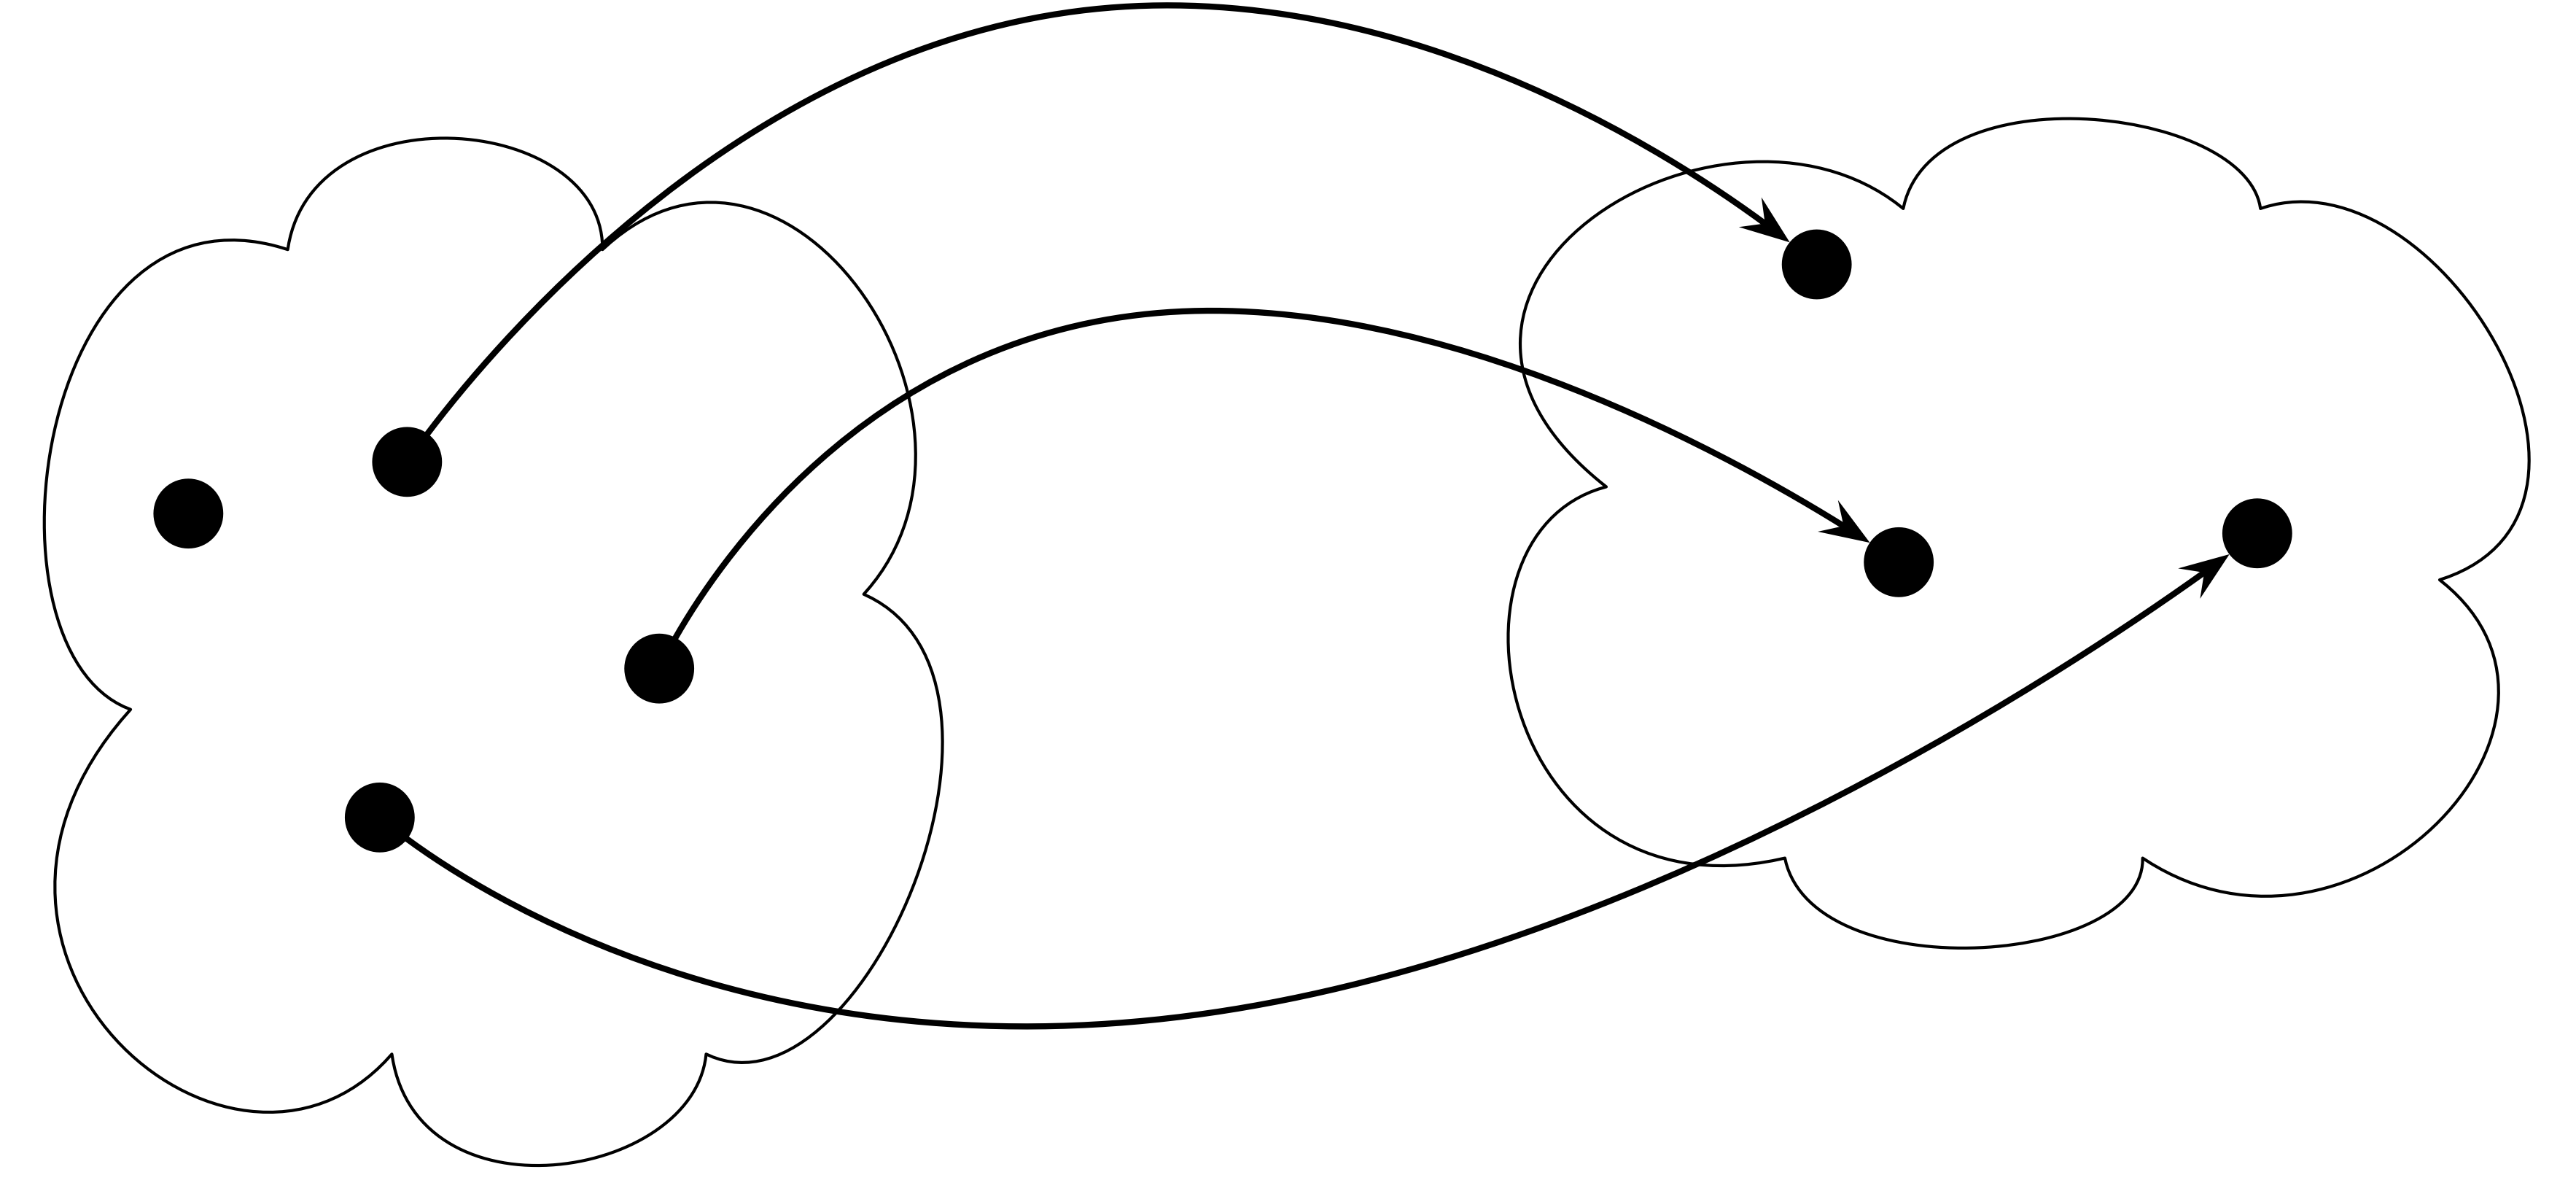
\includegraphics[width=.5\linewidth,right]{images/relations/surjection.png}
  \caption{Surjection.}
  \label{fig:surjection}
\end{figure}

\textbf{3.} The function \(f\) is a \textbf{bijection} if \(f\) is both injective and surjective. In other words, all elements of \(A\) are mapped uniquely to all elements of \(B\).

\begin{figure}
  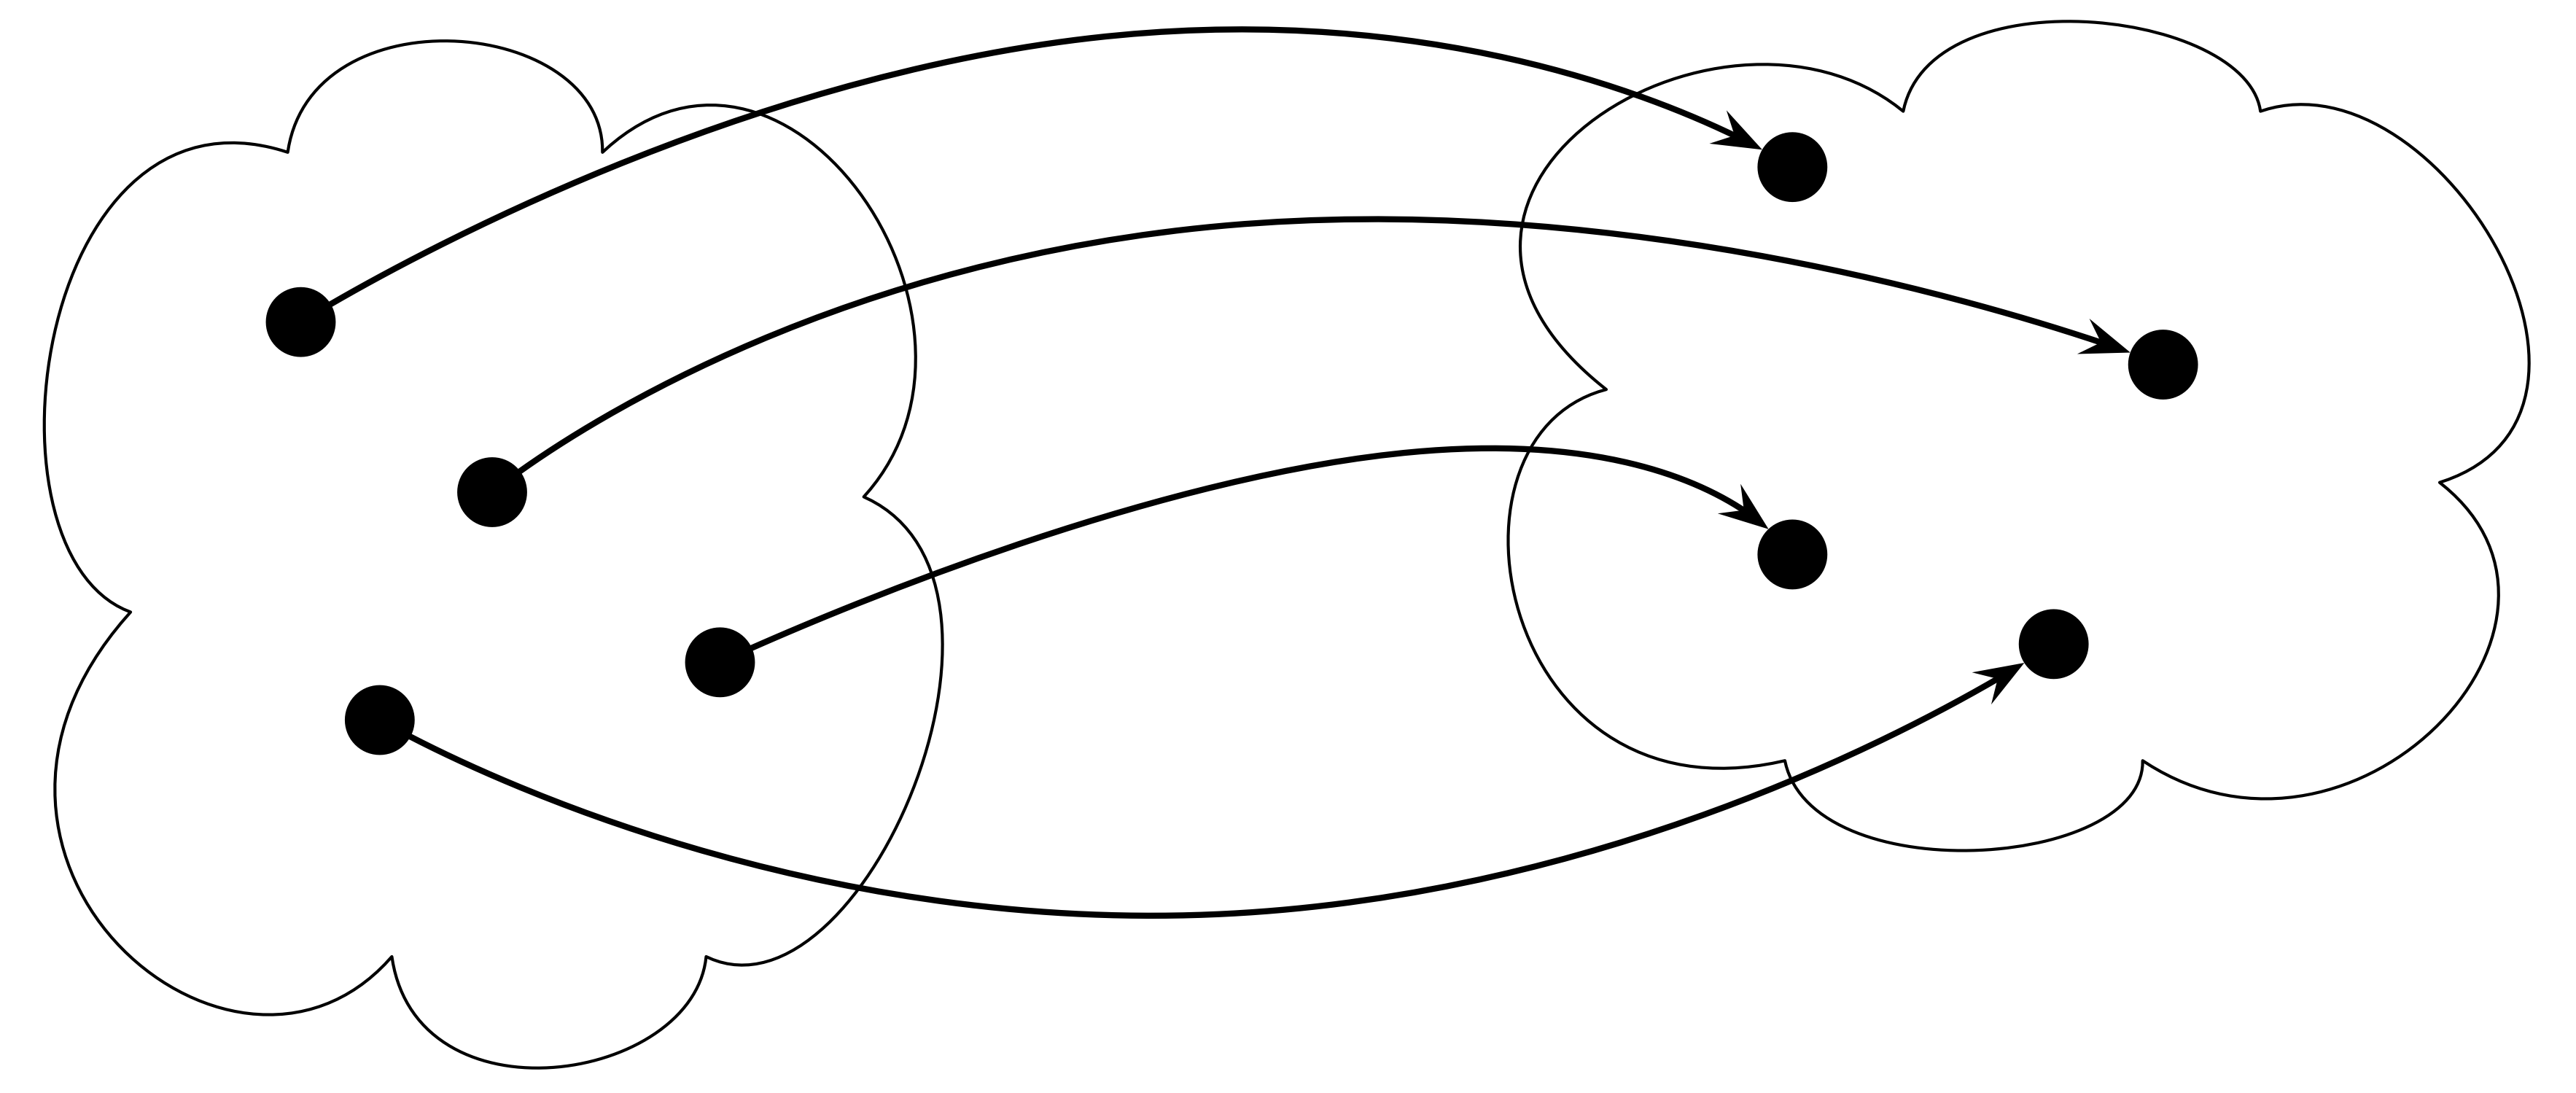
\includegraphics[width=.5\linewidth,right]{images/relations/bijection.png}
  \caption{Bijection.}
  \label{fig:bijection}
\end{figure}

We'll not focus on functions and relations anymore at the moment. Depending on how this course goes on, we'll either keep getting back to elements of this topic, or will extract it into a separate chapter.

\chapter{Proof techniques}
\label{sec:org4ff0fef}

\section{Direct proof}
\label{sec:org20add57}

Back when we've been discussing set cardinality, we've successfully proved a statement: \emph{If \(A\) is a finite set of \(m\) elements, then there are \(2^{m}\) subsets of \(A\).} Let's talk about proofs in more detail, and discuss different proof techniques.

A proof is a sequence of mathematical statements, a path from some basic truth to the desired outcome. An impeccable argument, if you will. Possibly the simplest form of proof is a direct proof. It's a straightforward attempt to see what the statement means if we dare to play with it. Consider a theorem:

\textbf{Theorem 1.} If \(n\) is an odd positive integer, then \(n^2\) is odd.

\textbf{Proof.} An odd positive integer can be written as \(n = 2k + 1\), since something like \(2k\) is even and adding 1 makes it definitely odd. We're interested in what odd squared looks like, so let's square this definition:

$$ n^2 = (2k + 1)^2 = $$
$$ 4k^2 + 4k + 1 = $$
$$ 2(2k^2 + 2k) + 1 $$

So, we have this final formula \(2(2k^2 + 2k) + 1\) and it follows the pattern of \(2k + 1\). This means it's odd! We have a proof. \(\blacksquare\)

(This black square — \(\blacksquare\) — is the symbol mathematicians often use to denote the end of proof.)

This theorem is based on an idea that numbers described as \(2k + 1\) are definitely odd. This idea could be another theorem that requires another proof, and that proof would be based on some other theorems. The general idea of mathematics is that if you follow any theorem to the very beginning, you'll meet the fundamental axioms, the basis of everything.

\section{Constructive proof}
\label{sec:org573604e}

The idea behind constructive proof is to show the existence of a certain object by describing a method of creating it.

\textbf{Theorem 2.} There exists a rational number \(x\) such that \(\sqrt{10^{100}} < x < \sqrt{10^{100}+1}\).

\textbf{Proof.} \(\sqrt{10^{100}}\) is \(10^{50}\). Now, let's just try different clearly rational values for \(x\) that \emph{seem} to lie between the required boundaries. For example, let's try \(x = 10^{50} + 10^{-51}\). It's obviously larger than \(10^{50}\), so we only need to show that it's smaller than \(\sqrt{10^{100}+1}\).

To do that, let's compute \(x^{2}\) so that we can compare it with \((\sqrt{10^{100}+1})^{2}\):

$$ x^{2} = (10^{50} + 10^{-51})^{2} $$
$$ = 10^{100} + 2 \times (10^{50} \times 10^{-51}) + 10^{-102} $$
$$ = 10^{100} + 2 \times 10^{50-51} + 10^{-102} $$
$$ = 10^{100} + 2 \times 10^{-1} + 10^{-102} $$

Clearly:

$$ (2 \times 10^{-1} + 10^{-102}) < 1 $$

therefore

$$ 10^{100} + 2 \times 10^{-1} + 10^{-102} < (\sqrt{10^{100}+1})^{2} $$
$$ x^{2} < (\sqrt{10^{100}+1})^{2} $$

and, by extension

$$ x < \sqrt{10^{100}+1} $$

Therefore, there indeed exists a rational number \(x\) such that \(\sqrt{10^{100}} < x < \sqrt{10^{100}+1}\) \(\blacksquare\).

\section{Proof by Contradiction}
\label{sec:org43b908d}

Another approach is proof by contradiction. Here is the idea:

\begin{enumerate}
\item Assume the statement is false or true.
\item Derive a contradiction, a paradox, something that doesn't make sense. This will mean that the statement cannot possibly be what we assumed it to be, therefore it's the opposite.
\end{enumerate}

When I first saw this formal technique, it puzzled me. It didn't seem to be valid: alright, assuming something is false leads to a paradox, so what? We haven't proven that assuming it's true doesn't lead to another paradox! Or even the same paradox, for that matter. What I failed to understand conceptually is that a statement is a binary thing: it's either true or untrue. Nothing in between. So, if one can definitely declare "X is not false", then no other options are left: "X must be true".

\textbf{Theorem 3.} \(n\) is a positive integer. If \(n^2\) is even, then \(n\) is even.

We may try to construct another direct proof, but creating paradoxes is much more fun!

\textbf{Proof.} Let's assume that \(n^2\) is even, \textbf{but \(n\) is odd}. This is the opposite of what we want, and we will show that this scenario is impossible.

\(n\) is odd, then, according to Theorem 1 (which is already proven), \(n^2\) must be odd. This doesn't make sense! Our assumption and our conclusion are the opposite. This is a paradox, so the assumption was wrong. Meaning, the idea "\(n^2\) is even, but \(n\) is odd" is false. Therefore, the idea "\(n^2\) is even, \(n\) is even" is true. \(\blacksquare\)

\noindent\rule{\textwidth}{0.5pt}

Let's look at one rather famous proof of irrationality of \(\sqrt{2}\).

\textbf{Theorem 4.} \(\sqrt{2}\) is irrational.

Woah, this is\ldots{} different. Prior theorems were formulas, something to play with, something physical. But here is just an idea, so how would we even start?

Let's start with a definition.

\begin{quote}
In mathematics, the irrational numbers are all real numbers which are not rational numbers.\footnote{\url{https://en.wikipedia.org/wiki/Irrational\_number}}
\end{quote}

Doesn't seem helpful, but let's continue. What are rational numbers then? Are they some reasonable beings who make optimal decisions all the time?

\begin{quote}
A rational number is any number that can be expressed as the fraction \(\frac{p}{q}\) of two integers.\footnote{\url{https://en.wikipedia.org/wiki/Rational\_number}}
\end{quote}

Oh! They are rational because they are \emph{ratios}! Just to make things super clear, let's dig one more step and make sure we understand integers.

\begin{quote}
An integer (from the Latin \emph{integer} meaning "whole") is a number that can be written without a fractional component. For example, \(21\), \(4\), \(0\), and \(−2048\) are integers, while \(9.75\), \(5\frac{1}{2}\) and \(\sqrt{2}\) are not.\footnote{\url{https://en.wikipedia.org/wiki/Integer}}
\end{quote}

Combining these things, we can construct a comprehensive definition of the irrational number: it's a number that cannot be expressed as the fraction of two whole numbers. Now, let's apply this to Theorem 3 so that it has some meat:

\textbf{Theorem 4, re-framed.} \(\sqrt{2}\) cannot be expressed as \(\frac{p}{q}\), where \(p\) and \(q\) are integers.

Alright, now there is something to play with!

\textbf{Proof.} Start by assuming the opposite: \(\sqrt{2}\) is rational. This means it can be written as a fraction of two integers:

$$ \sqrt{2} = \frac{p}{q}\ $$

We can assume that \(p\) and \(q\) are not \textbf{both} even, because if they are, we can reduce them by dividing both by a common factor (like, for example, \(\frac{8}{10}\\) should be reduced to \(\frac{4}{5}\\)). In other words, if they are both even, reduce them until at least one is odd and no further reductions are possible.

Now, let's square the square root:

$$ (\sqrt{2})^2 = \frac{p^2}{q^2}\ $$

$$ 2 = \frac{p^2}{q^2}\ $$

$$ p^2 = 2q^2 $$

Remember, something like \(2k + 1\) is odd, and \(2k\) is even. Here we see this pattern: \(p^2 = 2q^2\), which means that \(p^2\) is even (it consists of \emph{two} things).

Then, using Theorem 3, we can say that \(p\) is even as well, which means we can write \(p\) as \(p = 2k\). So:

$$ 2q^2 = p^2 = (2k)^2 $$

$$ 2q^2 = 4k^2 $$

Divide both by two:

$$ q^2 = 2k^2 $$

So, \(q^2\) is even. According to the same Theorem 3 it follows that \(q\) is even.

Let's summarize the two conclusions:

\begin{enumerate}
\item \(p\) is even.
\item \(q\) is even.
\end{enumerate}

Wait\ldots{} We made sure that not both \(p\) and \(q\) are even before starting this whole thing! We made sure to reduce them until at least one is odd, but then, by applying Theorem 3, we ended up with two even numbers. This is impossible, so the idea that "\(\sqrt{2}\) is rational" is not true.

Therefore, \(\sqrt{2}\) is irrational. \(\blacksquare\)

\section{Proof by Induction}
\label{sec:org0bc45f1}

One of the most powerful techniques is proof by induction.

\marginnote{Do not confuse mathematical induction with inductive or deductive reasoning. Despite the name, mathematical induction is actually a form of deductive reasoning.}

Let's say, we want to prove that some statement \(P\) is true for all positive integers. In other words: \(P(1)\) is true, \(P(2)\) is true, \(P(3)\) is true\ldots{} etc.

We could try and prove each one directly or by contradiction, but the infinite number of positive integers makes this task rather grueling. Proof by induction is a sort of generalization that starts with the basis:

\textbf{Basis:} Prove that \(P(1)\) is true.

Then makes one generic step that can be applied indefinitely. \textbf{Induction step:} Prove that for all \(n\geq1\), the following statement holds: If \(P(n)\) is true, then \(P(n+1)\) is also true.

We've devised another problem to solve, and it's seemingly the same. But if the basis is true, then proving this \emph{inductive step} will prove the theorem. To do this, we chose an arbitrary \(n\geq1\) and assumed that \(P(n)\) is true. This assumption is called the \emph{inductive hypothesis}. The tricky part is this: we don't prove the hypothesis directly, but prove the \(n+1\) version of it.

This is all rather amorphous, so let's prove a real theorem.

\noindent\rule{\textwidth}{0.5pt}

\textbf{Theorem 5.} For all positive integers \(n\), the following is true:

\begin{equation}
1 + 2 + \ldots + n = \frac{n(n+1)}{2}
\end{equation}

\textbf{Proof}. First, just calculate the basis when \(n = 1\):

$$ 1 = \frac{1(1+1)}{2} = \frac{2}{2}. $$

This is correct, so, the basis is proven. Now, assume that the theorem is true for any \(n\geq1\):

\begin{equation}
1 + 2 + \ldots + n = \frac{n(n+1)}{2}
\end{equation}

Holding that assumption, prove the induction step. In other words, prove that the basis is also true for \(n+1\):

\begin{equation}
1 + 2 + \ldots + (n+1) = \frac{(n+1)(n+2)}{2}
\end{equation}

\emph{(All we did is substituted \(n\) with \(n+1\).)}

We can expand this equation. The last member on the left side is \(n+1\). In front of it must be \(n\), so let's show it:

$$ 1 + 2 + \ldots + (n+1) $$
$$ = 1 + 2 + \ldots + n + (n+1)$$

Assumption (2) tells us the value of \(1 + 2 + \ldots + n\), so let's take it and replace the corresponding part of the right-hand side (rectangle shows this replacement):

$$ 1 + 2 + \ldots + (n + 1) = \boxed{ \frac{n(n+1)}{2} } + (n+1) $$

And then make that addition so that the right hand side is a single fraction:

$$ \frac{n(n+1)}{2} + \frac{2(n+1)}{2} $$
$$ = \frac{n(n+1) + 2(n+1)}{2} $$
$$ = \frac{(n+1)(n+2)}{2}. $$

So:

\begin{equation}
1 + 2 + \ldots + (n + 1) = \frac{(n+1)(n+2)}{2}
\end{equation}

Great, the've proved that the induction step (3) is true. So far, we have two results:

\begin{enumerate}
\item The theorem is true for \(n=1\).
\item If the theorem is true for any \(n\), then it's also true for \(n+1\).
\end{enumerate}

Note how neither of the two facts is sufficient alone. The first fact is limited to a single case. The second fact is based on a condition — it basically says "give me a ladder, then I can touch the sky". Fact 1 is the ladder. Now, we can touch the sky by combining the two facts. The theorem is true for all positive integers \(n\). \(\blacksquare\)

\noindent\rule{\textwidth}{0.5pt}

I had troubles with this technique because for a long time I couldn't for the life of me understand why is this \emph{enough} and how is the basis \emph{helping}?! The basis seemed redundant. We assume \(P(n)\) is true, then prove that \(P(n+1)\) is true given that \(P(n)\) is true, but so what? We didn't prove the thing we assumed!

It clicked after I understood that we don't have to prove \(P(n)\), we just take the concrete value from the basis and use it as \(n\). Since we have a proof of \(P(n+1)\) being true \textbf{if} \(P(n)\) is true, we conclude that if \(P(1)\) is true, then \(P(1+1)\) is true. Well, if \(P(1+1)\) is true, then, using the same idea, \(P(1+1+1)\) is true, and so forth.

The basis was the \emph{cheat-code} to kick-start the process by avoiding the need to prove the assumption (2).

\section{The pigeon hole principle}
\label{sec:org39cfd5d}

This is a simple, obvious principle with surprisingly powerful consequences. The pigeon hole principle is something toddlers learn: if you put 3 blocks into 2 boxes, one box will end up with more than 1 block.

Formally: if \(n+1\) or more objects are placed into \(n\) boxes, then there is at least one box containing two or more objects.

Now that we know about sets and functions, we can also compose the definition in terms of set theory: if \(A\) and \(B\) are two sets such that \(|A| > |B|\), then there is no one-to-one function from \(A\) to \(B\).

\textbf{Theorem 6.} Let \(n\) be a positive integer. Every sequence of \(n^{2}+1\) distinct real numbers contains a subsequence of length \(n+1\) that is either increasing or decreasing.

Example: let's take \(n = 3\). A sequence of \(3^{2}+1\) distinct real numbers could look like so: \((20, 10, 9, 7, 11, 2, 21, 1, 20, 31)\). According to the theorem, it must contain a subsequence of length \(3+1\). Look closely and, indeed, it does: \((10, 11, 21, 31)\).

\textbf{Proof.} Let \((a_{1}, a_{2}, \ldots ,a_{n^{2}+1})\) be an arbitrary sequence of \(n^{2}+1\) distinct real numbers. For each \(i\) with \(1 \leq i \leq n^{2} + 1\):

\begin{itemize}
\item let \(inc_{i}\) denote the length of the longest increasing subsequence that starts at \(a_{i}\)
\item let \(dec_{i}\) denote the length of the longest decreasing subsequence that starts at \(a_{i}\).
\end{itemize}

Let's reformulate the theorem using this notation: there is an index \(i\) such that \(inc_{i} \geq n+1\) \textbf{or} \(dec_{i} \geq n+1\).

We will prove this claim by contradiction, using the pigeon hole principle. Recall that proof by contradiction starts with the negation (opposite) of the theorem's claim. So, \textbf{assume} that \(inc_{i} \leq n\) and \(dec_{i} \leq n\) for all \(i\) with \(1 \leq i \leq n^{2} + 1\).

Now, consider the set:

$$ B = \{ (b,c) : 1 \leq b \leq n, 1 \leq c \leq n \}, $$

and think of elements of \(B\) as boxes. For each \(i\) with \(1 \leq i \leq n^{2} + 1\), the pair \((inc_{i}, dec_{i})\) is an element of \(B\). So we have \(n^{2} + 1\) such elements \((inc_{i}, dec_{i})\), but there are only \(n^{2}\) boxes in \(B\). By the pigeon hole principle, there must be a box that contains two or more elements. So, there exists two integers \(i\) and \(j\) such that \(i < j\) and

\begin{equation}
(inc_{i}, dec_{i}) < (inc_{j}, dec_{j}).
\end{equation}

Recall that the elements in the sequence are distinct (no repeating numbers). Hence, \(a_{i} \neq a_{j}\). There are two cases then:

\textbf{Case 1.} \(a_{i} < a_{j}\). Then the length of the longest increasing subsequence starting at \(a_{i}\) must be \(1 + inc_{j}\), because we can append \(a_{i}\) to the longest increasing subsequence starting from \(a_{j}\). Therefore, \(inc_{i} \neq inc_{j}\), which contradicts (1).

\textbf{Case 2.} \(a_{i} > a_{j}\). Then the length of the longest deccreasing subsequence starting at \(a_{i}\) must be \(1 + inc_{j}\), because we can append \(a_{i}\) to the longest deccreasing subsequence starting from \(a_{j}\). Therefore, \(dec_{i} \neq dec_{j}\), which again contradicts (1). \(\blacksquare\)

\part{Computational Complexity}
\label{sec:org7e33125}
\chapter{Intro to complexity}
\label{sec:orge22f2ad}

The proper way to discuss computational complexity would probably look like this: start with the idea of computation, describe models of computation (e.g. Turing machines and/or Lambda calculus), discuss limits of computation, explore automatons and languages (not programming languages, but formal languages derived from formal grammars like Context-free grammar), and then, finally, discuss the ways we can count the number of operations for certain algorithms.

Since this isn't an academic textbook (and we're busy developers), we will talk about computational complexity from the points of view of everyday programming. Nevertheless, the computability of the Universe, models of computations and their limits are very interesting and important (in that order!) topics. A separate chapter will focus on those.

You probably have at least a vague idea about algorithms. Often, analogies are used:

\begin{itemize}
\item meal recipe
\item walking directions
\item emergency situation instructions
\end{itemize}

It's important to distinguish between the general idea of an algorithm and the precise, formal, mathematical algorithms used in computer science. The ones above are \emph{examples} of regular, every-day algorithms. They aren't really analogies, but we don't think of them as algorithms, simply because they are too vague, open to interpretation. "Fry onions on medium heat until brown" — how brown is brown enough? what is medium heat? what exact light frequencies and temperatures are we talking about?!

The reason such instructions aren't extremely precise is that for the most part they're enough. The recipes are more like suggestions. People can make their own decisions and interpretations.

\begin{marginfigure}
  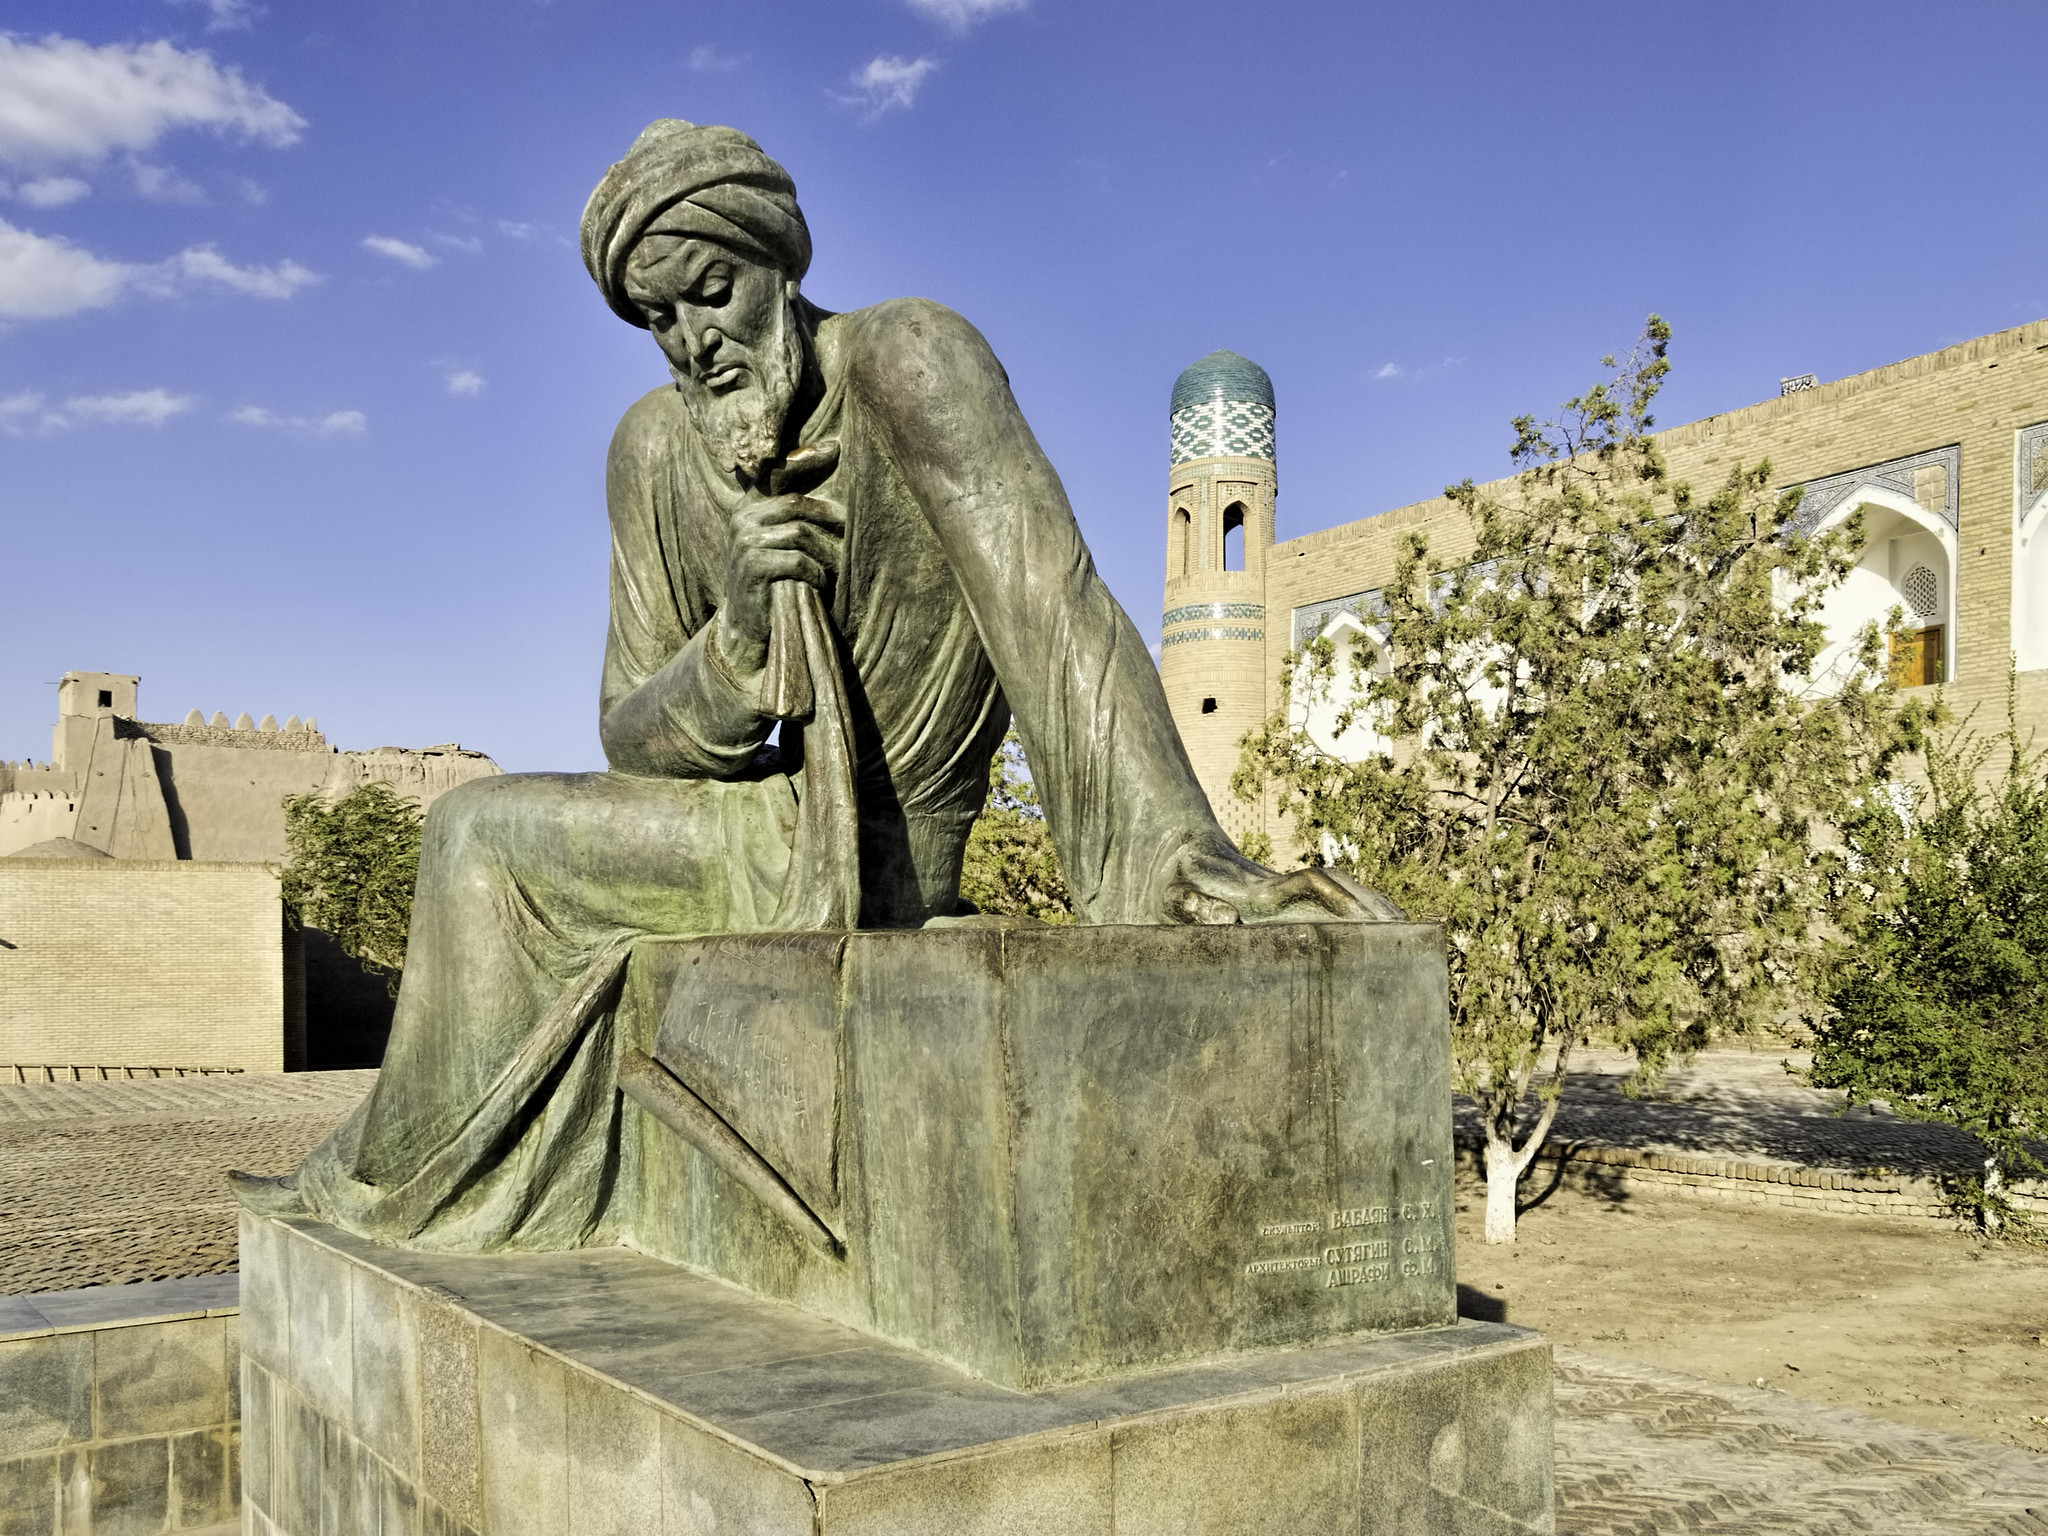
\includegraphics[width=\linewidth]{images/Muhammad ibn Musa al-Khwarizmi.jpg}
  \caption{Statue of Muhammad ibn Musa al-Khwarizmi, just outside Khiva’s west wall, Uzbekistan. Photo by Dan Lundberg.}
  \label{fig:marginfig}
\end{marginfigure}

But computers can't. Computers can only follow precise, unambiguous instructions. Yet, the roots of this formal nature of algorithms are much older than digital computers. The word "algorithm" itself was derived from the name of Muhammad ibn Musa al-Khwarizmi, a Persian scholar who lived in years 780-850. His books described algorithms for calculating certain numbers. These algorithms — instructions — must be precise and unambiguous even though they were created for mortal humans.
\chapter{Euclid's algorithm}
\label{sec:org3a0026c}

Let's start with the famous, ancient algorithm for finding the greatest common divisor (GCD) of two numbers. GCD is the largest number that divides both given numbers without leaving a remained. For example, GCD of 4 and 8 is 4.

Unless you know about Euclid's algorithm, stop and think for a while — how would you find a GCD of two numbers? What generic approach might work for any case (not taking efficiency into account for the time being)?

Right off the bat, one could suggest simply trying all the numbers from the largest-minus-one down to 1. That's certainly a fine way, and considering the enormous power of modern computers, will take a fraction of a second for even large-ish numbers. Euclid, of course, was trying to solve this about 2300 years before modern computers. Trying out all the numbers manually is the last resort for any computational task. Although, if you can prove that the only way to solve the problem at hand is by brute force, then that's a good result. Some problems are fundamentally hard, for example, finding an element in an unsorted collection: there is just no way to optimize anything, you have to check all the elements (in the general case).

The Euclid's algorithm is a series of simple computations. Let's say we want to find the GCD of two numbers \(a = 831, b = 47\). The first step is to divide the larger number by the smaller and find the quotient \(q_{0}\) and the remainder \(r_{0}\):

$$831 = q_{0} \times 47 + r_{0}$$
$$831 = 17 \times \underline{47} + \underline{32}$$

Next, repeat the process by taking the quotient as new \(a\) and remainder as new \(b\):

$$47 = q_{1} \times 32 + r_{1}$$
$$47 = 1 \times \underline{32} + \underline{15}$$

And again:

$$32 = q_{2} \times 15 + r_{2}$$
$$32 = 2 \times \underline{15} + \underline{2}$$

And again:

$$15 = q_{3} \times 2 + r_{3}$$
$$15 = 7 \times \underline{2} + \underline{1}$$

And finally, we reach the remainder = \(0\):

$$2 = q_{4} \times 1 + r_{4}$$
$$2 = 2 \times 1 + 0$$

This series is guaranteed to end with a zero remainder, and the last non-zero remainder is the greatest common divisor (we won't provide a proof here for either statements). In our example, \(GCD(831, 47) = 1\).

This is a proper algorithm because:
\begin{itemize}
\item It is formal and unambiguous. There is no room for interpretation or assumption.
\item It can be proved to we correct.
\item It can be analyzed, best and worst case scenarios can be determined for the general case.
\end{itemize}

Let's implement this algorithm in Python.

\begin{verbatim}
def gcd(a, b):
  while b != 0:
    t = b
    b = a % b
    a = t
  return a
\end{verbatim}

It's a recursive approach, which is a natural idea under given circumstances, since each step of the Euclid's algorithm is the same, only the numbers "shift". The stopping condition is \texttt{b != 0}, and until it's reached we use \texttt{t} as a temporary variable while computing new value for \texttt{b}. Recall that \texttt{\%} is a modulo operator which returns the remainder after division — exactly what we need for \(r_{k}\) at each step \(k\).
\chapter{Analyzing Euclid's algorithm: statistical observations}
\label{sec:org9d82481}

Let's now try to analyze Euclid's algorithm, or, rather, this particular implementation in Python:

\begin{verbatim}
def gcd(a, b):
  while b != 0:
    t = b
    b = a % b
    a = t
  return a
\end{verbatim}

We're interested in the algorithm itself, so let's ignore any caveats, details or optimizations of the Python interpreter.

What is there to analyze? What can we count? Let's zoom out and think about the purpose of such analysis.

Analyzing a single algorithm doesn't seem useful. Let's say we've figured out that it takes \(N\) loop iterations. So? Is this information useful or actionable? Not really. It makes sense to analyze so that we can \emph{compare} different algorithms. If Euclid's algorithm takes \(N\) actions, while some other Algorithm X takes \(N/2\) actions, then clearly, the other algorithm is better!

\textbf{Purpose of algorithm analysis 1: to compare algorithms.}

Another purpose is to compare the algorithm to itself with different inputs. Obviously, we're not fundamentally interested in the complexity of calculating GCD of 47 and 831. We're interested in the complexity of calculating \emph{any} GCD. This means we need to think about how one input compares to another input. In other words, how would the number of actions increase change when inputs change.

\textbf{Purpose of algorithm analysis 1: to evaluate the scalability of the algorithm.}

Now, loop iterations are too vague of a measure. We need to count something more concrete and fundamental enough so that any algorithm can be thought of as a combination of such operations. Atomic operations, if you will. There are different ways to chose which operations to consider atomic. A common way is to think about real CPUs and RAM. In the context of digital computing and \href{https://en.wikipedia.org/wiki/Von\_Neumann\_architecture}{Von Neumann architecture}, the atomic operations could be:

\begin{itemize}
\item arithmetic operations \texttt{+}, \texttt{*}, \texttt{-}
\item comparison of values using \texttt{=}
\item accessing memory
\item writing into memory
\item loops steps, subroutine calls, function calls, conditionals
\end{itemize}

This approach is called The RAM Model of Computation. It approximates what the computer does, but is not precise. It is useful for our two purposes, but it's not a way to measure the performance of computer programs.

How many atomic steps happen in a single loop iteration of \texttt{gcd}?

\begin{verbatim}
t = b      # 1 memory read + 1 write
b = a % b  # 1 calculation + 1 memory write
a = t      # 1 memory read + 1 write
\end{verbatim}

6 in total. It's a small number, could've been 100 for some other algorithm, but it is insignificant due to its static nature, not its value. Any given iteration will have 6 operations, regardless of the size of the input numbers. So, for the most part, we can ignore this particular number and instead think about the thing that changes when input changes. That thing is the number of loop iterations.

First, let's consider possible scenarios:

\begin{enumerate}
\item \texttt{gcd(0,0)}. No steps, yields \texttt{0}. Not interesting for our purposes.
\item \texttt{gcd(a,0)} or \texttt{gcd(0,b)}. No steps, yields \texttt{a} or \texttt{b}. Not interesting for our purposes.
\item \texttt{gcd(a,1)} or \texttt{gcd(1,b)}. 1 step, yields \texttt{1}.
\item \texttt{gcd(a,b)} where one is the multiple of the other. 2 steps, yields the smaller number.
\item \texttt{gcd(a,b)} where one is not the multiple of the other.
\end{enumerate}

Cases 3 and 4 are interesting, because the number of steps is fixed regardless of the input, as long as the input numbers satisfy the given conditions. Case 5 is the general case, which includes the worst possible combination of inputs.

Cases 1,2,3,4 describe the best scenarios. It doesn't matter that some perform 0 steps while others perform 1 step. What's important is that all cases have constant number of steps regardless of the input. They are \textbf{\textbf{constant time cases}}.

An algorithm that always works in constant time is the best possible thing. For example, getting a random element from an array is a constant time operation (unless we want true randomness, which makes things more complicated).

Case 5 on the other hand describes the non-best scenarios. The number of steps depends on the inputs. The important question is \textbf{how}? The mathematical answer to this question is exactly what we want for the second purpose of analysis: determining scalability.

Let's consider the example we've covered before: \(GCD(831,47)\). From our step-by-step description, we know it took 5 steps (from 0 to 4) to determine the answer. Could it be worse? Let's put in the counter into the loop and observe a few examples:

\begin{verbatim}
def gcd(a,b):
  count = 0
  while b != 0:
    t = b
    b = a % b
    a = t
    count+= 1
  print(count)
  return a

gcd(831, 47)  # 5
gcd(831, 48)  # 3
gcd(831, 49)  # 5
gcd(831, 50)  # 8
gcd(831, 51)  # 4
gcd(831, 52)  # 3

gcd(196418, 121391) # 14
gcd(196418, 121392) # 16
gcd(196418, 121393) # 25
gcd(196418, 121394) # 16
gcd(196418, 121395) # 23
gcd(196418, 121396) # 14
\end{verbatim}

Firstly, when changing one number slightly, the amount of steps doesn't change dramatically. It kind of hangs around some fixed point. Secondly, when the numbers are significantly bigger, the amount of steps is not significantly larger. The largest we've seen so far is 25 steps for \texttt{a=196418}, \texttt{b=121393}.

These sorts of experimental observations don't usually lead to the answer, but at least can give a basis for assumption. Here we can assume that the number of steps does rise with the input numbers, but slowly. The rise is not linear.
\chapter{Analyzing Euclid's algorithm: observing growth}
\label{sec:orgc6b38f4}

Let's focus on the growth of steps.

The process repeats recursively until \texttt{b} is zero, so the slower \texttt{b} decreases, the more steps there are. Thus, we can re-frame the question "what is the worst input numbers?" into "what input numbers produce the slowest decrease of \texttt{b} over time?".

At each step, new \texttt{b} is calculated as \texttt{a \% b}, and new \texttt{a} takes the previous value of \texttt{b}. Let's add some prints into the program so that we can see the calculations at each step:

\begin{verbatim}
def gcd(a,b):
  while b != 0:
    q = int((a - (a%b)) / b)
    print(f"{a} = {q} × {b} + {a%b}")

    t = b
    b = a % b
    a = t

  return a

gcd(831, 47)
\end{verbatim}

\begin{verbatim}
831 = 17 × 47 + 32
47 = 1 × 32 + 15
32 = 2 × 15 + 2
15 = 7 × 2 + 1
2 = 2 × 1 + 0
\end{verbatim}

Compare this to the calculations we've performed manually earlier:

$$831 = 17 \times \underline{47} + \underline{32}$$
$$47 = 1 \times \underline{32} + \underline{15}$$
$$32 = 2 \times \underline{15} + \underline{2}$$
$$15 = 7 \times \underline{2} + \underline{1}$$
$$2 = 2 \times 1 + 0$$

Notice how \texttt{q} (quotient) changes: at first, it's \texttt{17}, which dramatically reduces the value for the next \texttt{a}. Then \texttt{q} is 1, 2, 7 and finally 2. Compare this to running \texttt{gcd(144, 89)}:

\begin{verbatim}
144 = 1 × 89 + 55
89 = 1 × 55 + 34
55 = 1 × 34 + 21
34 = 1 × 21 + 13
21 = 1 × 13 + 8
13 = 1 × 8 + 5
8 = 1 × 5 + 3
5 = 1 × 3 + 2
3 = 1 × 2 + 1
2 = 2 × 1 + 0
\end{verbatim}

Here, each quotient is \texttt{1}, the smallest possible value. That makes \texttt{a} decrease slower. The slowest, actually. This is the worst case. Thus, we can reframe the question once again:

\begin{enumerate}
\item "What are the worst input numbers?"
\item → "What input numbers produce the slowest decrease of \texttt{b} over time?"
\item → \textbf{"What input numbers make all quotients be \texttt{1}?"}
\end{enumerate}

Look at the previous output listing again. Do you notice something weird about values of \texttt{a}? 144, 89, 55, 34, 21, 13, 8, 5, 3, 2\ldots{} They are reversed Fibonacci numbers!

Fibonacci sequence is a recursively defined sequence of whole numbers:

$$F_{1} = 1$$
$$F_{2} = 1$$
$$F_{n} = F_{n-1} + F_{n-2}$$

So, the first several numbers are:

$$1, 1, 2, 3, 5, 8, 13, 21, 34, 55, 89, 144,...$$

Any \(F_{n}\), where \(n>2\), consists of two previous numbers \(F_{n-1}\) and \(F_{n-2}\). By definition, \(F_{n-1} > F_{n-2}\). Thus, \(F_{n-1}\) can divide \(F_{n}\) only once, which makes the quotient to be 1.

Turns out, if you start \(GCD\) with a pair of adjacent (consecutive) Fibonacci numbers, the quotient will be \(1\) at each step, and values of \(a\) will follow Fibonacci sequence. Moreover, the greatest common divisor of two adjacent Fibonacci numbers is always \(1\). That is to say, \textbf{\textbf{two adjacent Fibonacci numbers are coprime}} (prime with respect to each other).

We won't spend more time in this topic and will omit the proofs of these statements right now. The plan is to provide omitted proofs in the end of the book.

For now, we can take advantage of the fact that Fibonacci sequence is thoroughly explored by mathematicians. The growth rate of Fibonacci numbers with respect to \(n\) is exponential, and is asymptotic to

$$\varphi ^{n}/{\sqrt {5}}$$

where

$$\varphi=\frac {1+\sqrt {5}}{2} \approx 1.61803$$

is the \href{https://en.wikipedia.org/wiki/Golden\_ratio}{golden ratio}. For sufficiently large \(n\):

$$n \approx \frac { \log_{2} F_n}{\log_{2} \varphi}$$

This slightly difficult result is based on several assumptions and omitted proofs. Before continuing to the conclusion in the context of formal algorithmic complexity analysis, let's take a simpler detour into sorting algorithms. There, through a primitive scenario, we'll discuss the notion of upper bounds and Big O. And afterwards, we'll come back and finish analyzing Euclid's algorithm properly.
\chapter{Faithsort and Bogosort}
\label{sec:org6820219}

Sorting is the staple of computer science education. We all have to deal with sorting one way or another: in college, in textbooks or during job interviews. We also occasionally sort things in real life: books on the shelf by author or, perhaps, by color; tasks in our ToDo lists by importance or priority, etc. Yet, I don't think I had implemented a sorting algorithm in a professional setting, ever. And I can imagine only a small subset of programmers who think deeply about sorting and implement new or modified sorting algorithms as part of their job.

The reason people give sorting this much attention is twofold:

\begin{enumerate}
\item It is a truly important kind of problem in computer science.
\item Understanding and implementing sorting algorithms is a good exercise for computational thinking.
\end{enumerate}

Let's take an example collection of numbers \texttt{[3, 8, 1, 2, 5, 6, 4, 7, 9]} and see what approaches we can take.

What is the dumbest sorting algorithm possible? One idea is to check whether the collection is sorted, and if not, just wait and check again later. Of course, it will never be sorted. Or will it? Maybe with enough time in an infinite universe, bits could spontaneously flip due to quantum effects. Or, if we're talking on a more practical level, the electronic representation of said bits (computer memory) could be affected by cosmic rays, radiation or just plain data corruption. As a result, the possibility of the collection becoming sorted by accident is non-zero.

Let's call it "faithsort":

\begin{verbatim}
def faithsort(collection):
    while not is_sorted(collection):
        time.sleep(random.random())
    return collection
\end{verbatim}

How long would it take to successfully finish?

\begin{enumerate}
\item Best case: collection is empty or already sorted. Time needed: effectively 0.
\item Average case: collection becomes sorted after some time. Time needed: unknown, but finite.
\item Worst case: collection is never sorted. Time needed: n/a.
\end{enumerate}

Alright, jokes aside, what is the dumbest but still practical sorting algorithm possible? It's probably bogosort: shuffle the collection until it's sorted:

\begin{verbatim}
def bogosort(collection):
    while not is_sorted(collection):
        random.shuffle(collection)
    return collection
\end{verbatim}

How long would it take to successfully finish?

\begin{enumerate}
\item Best case: collection is empty or already sorted. Time needed: effectively 0.
\item Average case: collection becomes sorted after some shuffling. Time needed: unknown, but finite.
\item Worst case: collection is never sorted. Time needed: n/a.
\end{enumerate}

You can say that both faithsort and bogosort are equally useless, but it looks like with bogosort it's at least not inconceivable to expect the correct result in our lifetime. In fact, for our collection \texttt{[3, 8, 1, 2, 5, 6, 4, 7, 9]}, the Python program presented above was successful on average with ≈100000 permutations and took about 2-5 seconds on a modern laptop.

Both algorithms are bad not because they are slow, but mainly because they are \textbf{unbounded}: their worst case is infinity. This means we can't ever rely on the program to terminate (finish executing).

\noindent\rule{\textwidth}{0.5pt}

Consider a slightly better version: deterministic bogosort. In this version, the shuffling is not completely random, but instead it iterates through all possible permutations. The amount of permutations is finite if the collection is finite.

How to determine the number of permutations of \(n\) items? An intuitive explanation is rather simple. Consider nine elements \texttt{1, 2, 3, 4, 5, 6, 7, 8, 9}. Now, try to construct one permutation.

\begin{enumerate}
\item You need to choose the first element for it. There are 9 to choose from, so you have 9 choices.
\item Next, you need to chose the second element. There are 8 left to choose from.
\item Next, third element. 7 left to choose from.
\item Etc.
\end{enumerate}

So, the total number of permutations is \(9\times8\times7\times6\times5\times4\times3\times2\times1\) which is \(9!\) Thus, for \(n\) items, there are \(n!\) permutations.

Our deterministic bogosort does two things for each iteration: checks whether the collection is sorted and, if needed, shuffles it. We know there are at least \(n!\) permutations to shuffle through, so now we have to find out how much more work needs to happen for each permutation. This work is hidden in the checking (\texttt{is\_sorted(collection)}). How much work?

(Note: of course, the deterministic shuffling itself is a non-trivial task that would also require some work and contribute to the total number of operations. For simplicity, we're ignoring this part.)

Again, consider collection \texttt{1, 2, 3, 4, 5, 6, 7, 8, 9}. In order to determine whether it's sorted or not, you have to go through all the items and check that they're placed in increasing order. Best case is something like \texttt{9, 1, 2, 3, 4, 5, 6, 7, 8}: the first check immediately yields "not sorted". Worst case is something like \texttt{2, 3, 4, 5, 6, 7, 8, 9, 1}: you have to iterate through all the items and only at the last step it turns out the collection is not sorted.

So, worst case is \(n-1\) checks for the collection of \(n\) elements. If you want to go deeper, you can calculate the exact number of operations according to the RAM model: comparing a pair means accessing two elements (\(2\)), running a comparison operator (\(1\)), reading, increasing and writing the loop counter (\(1 + 1 + 1\)), etc. But, as you probably already noticed, we're not interested in accuracy as much as in scale. We can safely say it requires about \(n\) operations to check for sortedness, and ignore whatever constant multiplier there could be (like \(19 \times n\) — we don't care about 19, it's a constant number which never grows with \(n\)).

So, in total, deterministic bogosort requires \(n \times n!\) operations. This is its upper bound. Now the cases are as follows:

\begin{enumerate}
\item Best case: collection is empty or already sorted. Time needed: effectively \(0\).
\item Average case: collection becomes sorted after some shuffling. Time needed: unknown, but finite.
\item Worst case: collection becomes sorted after maximum possible amount of shuffling. Time needed: \(n \times n!\)
\end{enumerate}

Now it's bounded! Great!
\chapter{Bubble sort}
\label{sec:org15784ca}

Let us now talk about a more sensible algorithm for sorting. It's called Bubble sort. The idea is as follows:

\begin{enumerate}
\item Starting from the beginning, compare adjacent elements and swap them if needed.
\item Repeat until the list is sorted.
\end{enumerate}

Bubble sort is named like that because elements "bubble up" like in boiling water.

Our collection \texttt{[3, 8, 1, 2, 5, 6, 4, 7, 9]} would be sorted like this (elements currently compared are in bold):

First pass:

\begin{enumerate}
\item\relax [ \textbf{3, 8}, 1, 2, 5, 6, 4, 7, 9 ] (no swap)
\item\relax [ 3, \textbf{8, 1}, 2, 5, 6, 4, 7, 9 ] (swap)
\item\relax [ 3, 1, \textbf{8, 2}, 5, 6, 4, 7, 9 ] (swap)
\item\relax [ 3, 1, 2, \textbf{8, 5}, 6, 4, 7, 9 ] (swap)
\item\relax [ 3, 1, 2, 5, \textbf{8, 6}, 4, 7, 9 ] (swap)
\item\relax [ 3, 1, 2, 5, 6, \textbf{8, 4}, 7, 9 ] (swap)
\item\relax [ 3, 1, 2, 5, 6, 4, \textbf{8, 7}, 9 ] (swap)
\item\relax [ 3, 1, 2, 5, 6, 4, 7, \textbf{8, 9} ] (no swap)
\end{enumerate}

Second pass:

\begin{enumerate}
\item\relax [ \textbf{3, 1}, 2, 5, 6, 4, 7, 8, 9 ] (swap)
\item\relax [ 1, \textbf{3, 2}, 5, 6, 4, 7, 8, 9 ] (swap)
\item etc\ldots{}
\end{enumerate}

One pass takes about \(n\) steps, where \(n\) is the number of elements. Again, in reality it takes \(k \times n\) steps, where \(k\) is some constant (read/compare/write operations), but we don't care about it, since this number does not grow with the collection. The question is how many passes do we need?

Best case is one pass, because if the collection is already sorted, one pass is necessary to recognize this and halt. The worst case is when the collection is sorted backwards. This effective means that the last element must be swapped all the way down to the first position. That element can only travel one step backwards per one pass, so it takes \(n\) passes. In total, there are \(n\) passes, each with \(n\) swaps.

\begin{enumerate}
\item Best case: collection is empty or already sorted. Time needed: \(n\).
\item Average case: collection becomes sorted after some passes. Time needed: unknown, but finite.
\item Worst case: collection becomes sorted after maximum possible amount passes. Time needed: \(n \times n\) or \(n^{2}\).
\end{enumerate}

\chapter{Big O}
\label{sec:org4c3be2d}

When discussing average and worst case scenarios, we were interested in one thing which can be generalized as a question: "what is the upper bound (limitation) on the number of steps with respect to the size of the problem?" At the same time, we did not care about being super precise.

Big O notation is the tool for this task. It's a mathematical notation that describes the limiting behavior of a function as the argument grows. It is a member of a family of notations invented by Paul Bachmann, Edmund Landau and others, collectively called Bachmann–Landau notation or asymptotic notation.

Let's imagine some function \(f(n)\) which describes the growth of the number of operations required for some algorithm.

\begin{figure*}[htbp]
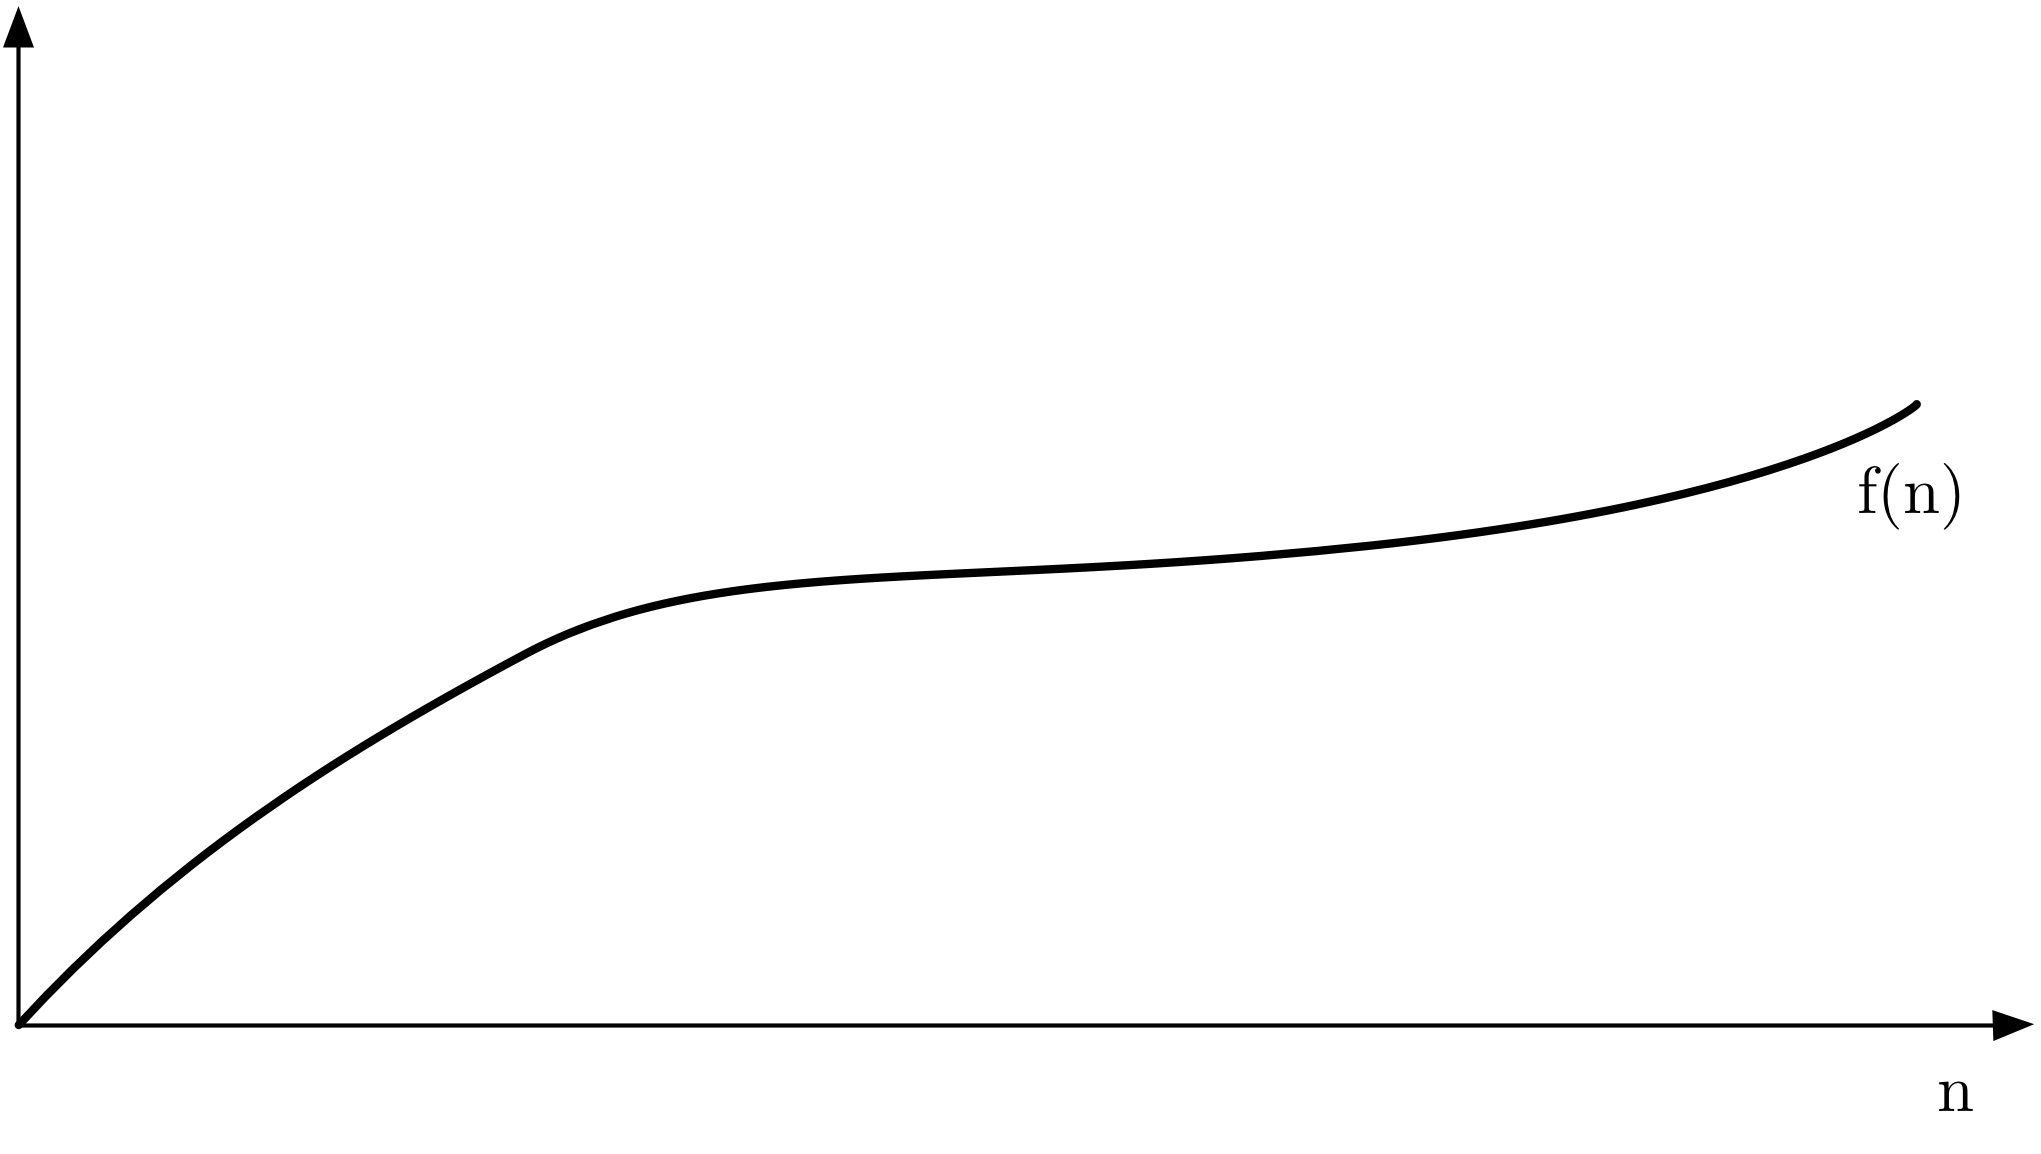
\includegraphics[width=.5\linewidth]{./images/big_o_theta_etc/fn.png}
\caption{\label{}
Graph of f(n).}
\end{figure*}
Now consider three additional things:

\begin{enumerate}
\item Some sufficiently large \(n\) (call it \(n_{0}\));
\item some other function \(g(n)\).
\item some number \(k\),
\end{enumerate}

so that:

$$ \lvert f(n) \rvert \leq k g(n) \textrm{ for all } n \geq n_{0} $$

In other words, \(g(n)\) multiplied by some number \(k\) is always "above" \(f(n)\) for sufficiently large \(n_{0}\).

\begin{figure*}[htbp]
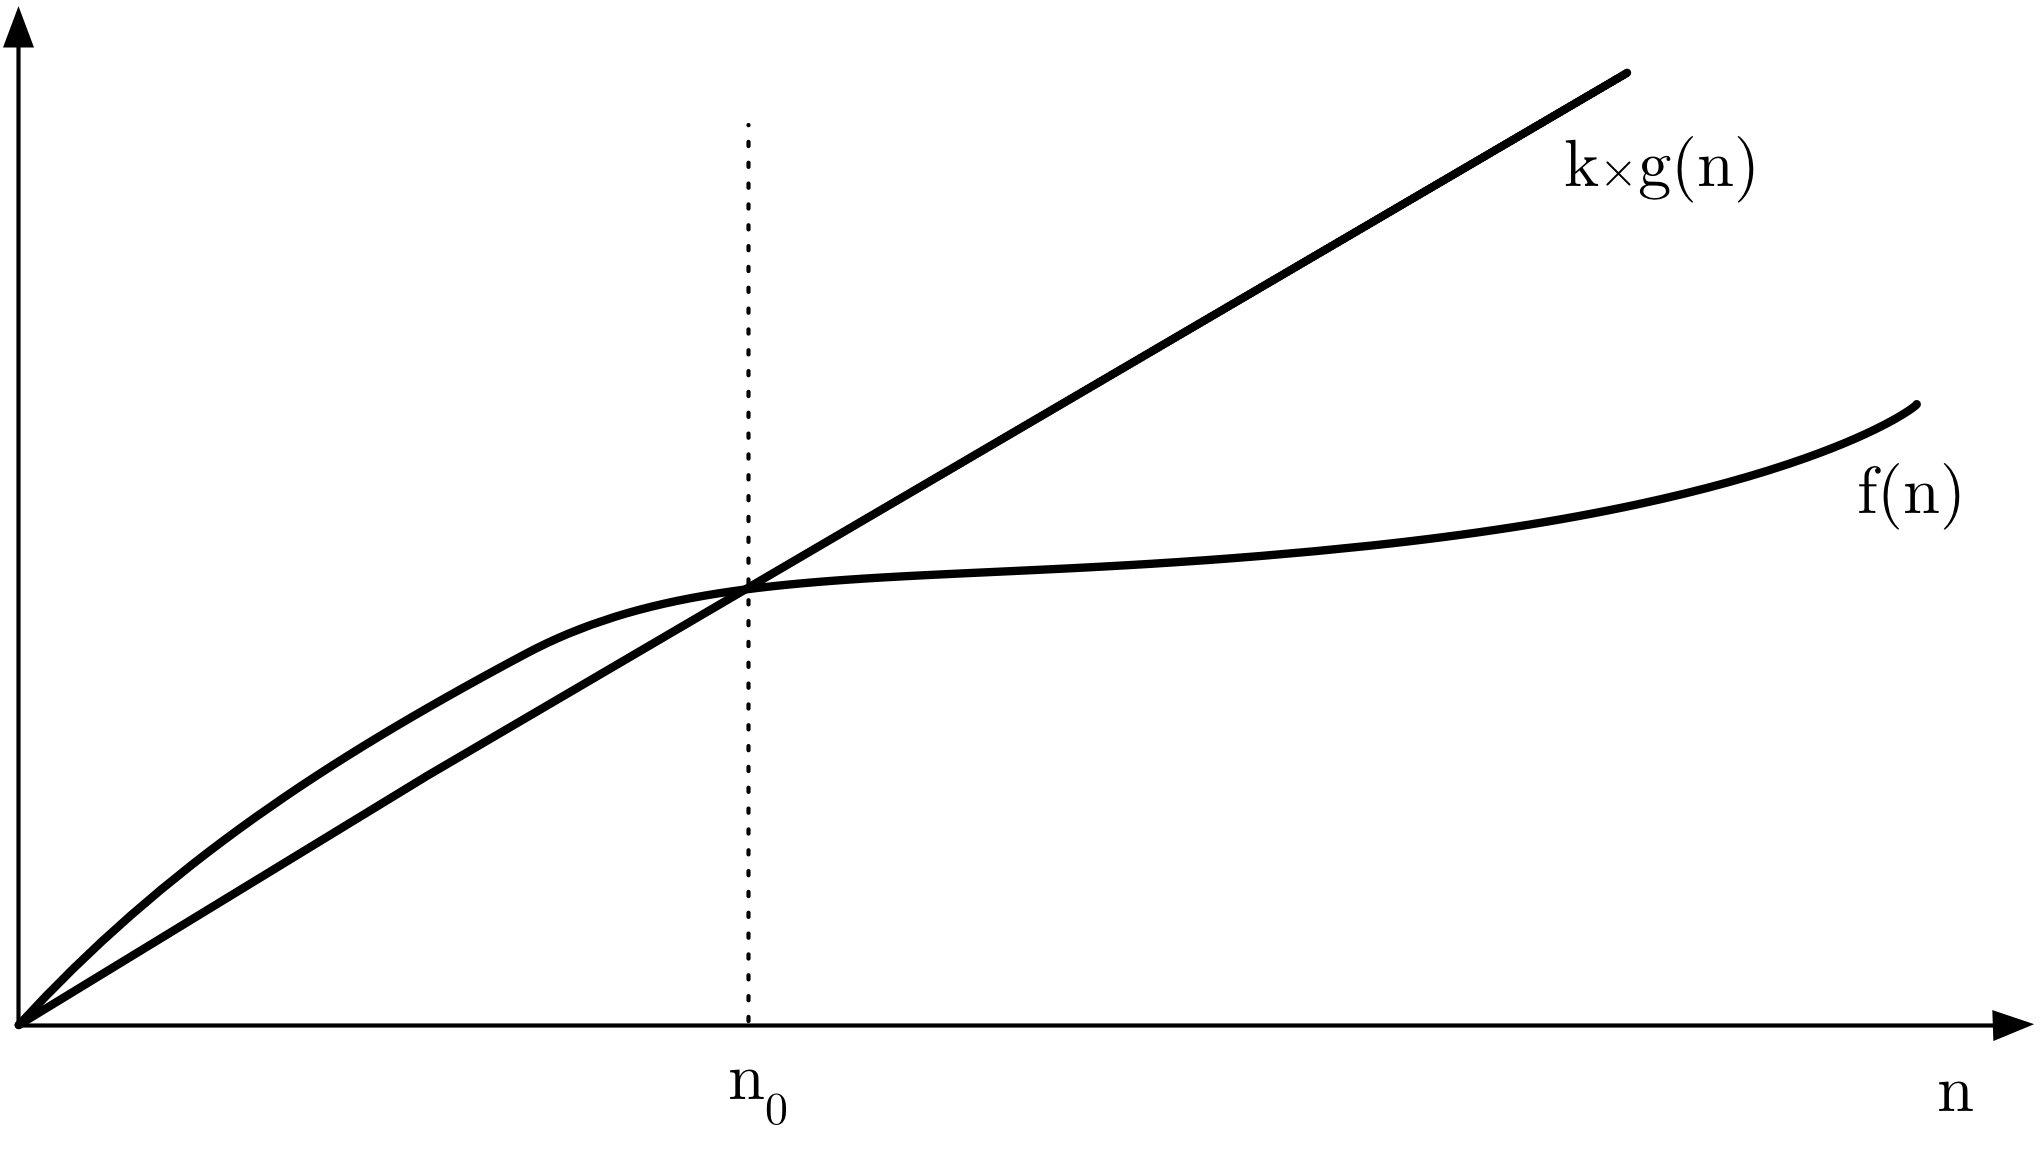
\includegraphics[width=.5\linewidth]{./images/big_o_theta_etc/fn and gn.png}
\caption{\label{}
Graphs of f(n) and g(n).}
\end{figure*}
If such function and values of \(k\) and \(n_{0}\) indeed exist, then we can say:

$$ f(n) = \mathcal{O}(g(n)) $$

That is the definition of Big O. A function is said to be Big O when it limits the other function as described above. The letter O was chosen because the notation is supposed to indicate the \textbf{order of the function}.

\marginnote{Often, instead of $f(n) = \mathcal{O}(g(n))$ computer scientists write $f(n) \textrm{ is } \mathcal{O}(g(n))$
because equality symbol there doesn't truly mean equality. Knuth describes such statements as "one-way equalities", since if the sides could be reversed, "we could deduce ridiculous things like $n = n^{2}$ from the identities $n = \mathcal{O}(n^{2})$ and $n^{2} = \mathcal{O}(n^{2})$.}

Recall what we had concluded about several algorithms discussed so far:

\begin{enumerate}
\item Euclid's algorithm: worst case is linked to Fibonacci sequence, the growth of which is asymptotic to \(\varphi ^{n}/{\sqrt {5}}\).
\item Deterministic bogo sort: worst case \(n \times n!\).
\item Bubble sort: worst case \(n^{2}\).
\end{enumerate}

We can now say that

\begin{enumerate}
\item Euclid's algorithm has time complexity of \(\mathcal{O}(log(n))\).
\item Deterministic bogo sort: \(\mathcal{O}(n \times n!)\).
\item Bubble sort: \(\mathcal{O}(n^{2})\).
\end{enumerate}

\chapter{Lower bounds for sorting. Big Omega (\(\Omega\))}
\label{sec:org75f05b5}

Generally speaking, for sorting, \(\mathcal{O}(n^{2})\) complexity is not great. Quadratic function grows very fast. Before exploring an alternative, better sorting algorithm, it makes sense to investigate the lower bounds for sorting. What is the best possible time complexity we can dream of?

Of course, ideally, we want all algorithms to be \(\mathcal{O}(1)\) — constant time. Which means that the algorithm yields correct solution in the same amount for time for any possible input. Note that this doesn't necessarily mean "fast". It could be that it takes trillions of operations and billions of years on a real computer, but the point is that it takes that much for any input, regardless of size. Let's see what the real lower bound is.

Bubble sort and other canonical algorithms are comparison-based: they compare pairs of elements in order to determine their relative position. As a result, the algorithm must output a permutation (rearrangement) of the input. For a collection of \(n\) elements, there are \(n!\) distinct permutations (recall the way permutations are calculated in "Faithsort and Bogosort"). For each of these permutations, there exists an input for which that permutation is the only correct answer. For example, the permutation \([a_{4}, a_{1}, a_{3}, a_{2}]\) is the only correct answer for the input \([9, 2, 7, 5]\). In fact, there exists a bijection (1-to-1 mapping) between different orderings of \(n\) distinct elements and the permutations needed to sort them. Give this, we can fix a set of \(n!\) inputs, one for each of \(n!\) output permutations.

Initially, the comparison-based sorting algorithm "knows" of \(n!\) possible correct permutations. In the end, it needs to settle on the one correct permutation. We can view the algorithm "travelling" from the first state to the last state, narrowing down the set of permutations all the way to one. The narrowing happens due to comparisons; each new comparison reduces the space of possible solutions. So, the computation can be thought of as a series of YES/NO questions, which yields a binary search tree. The root of the tree corresponds to the initial state of \(n!\) possible correct permutations, before any YES/NO questions is answered. One leaf of the tree corresponds to the correct permutation. For each possible input of size \(n\), there is a "correct leaf".

\begin{figure*}[htbp]
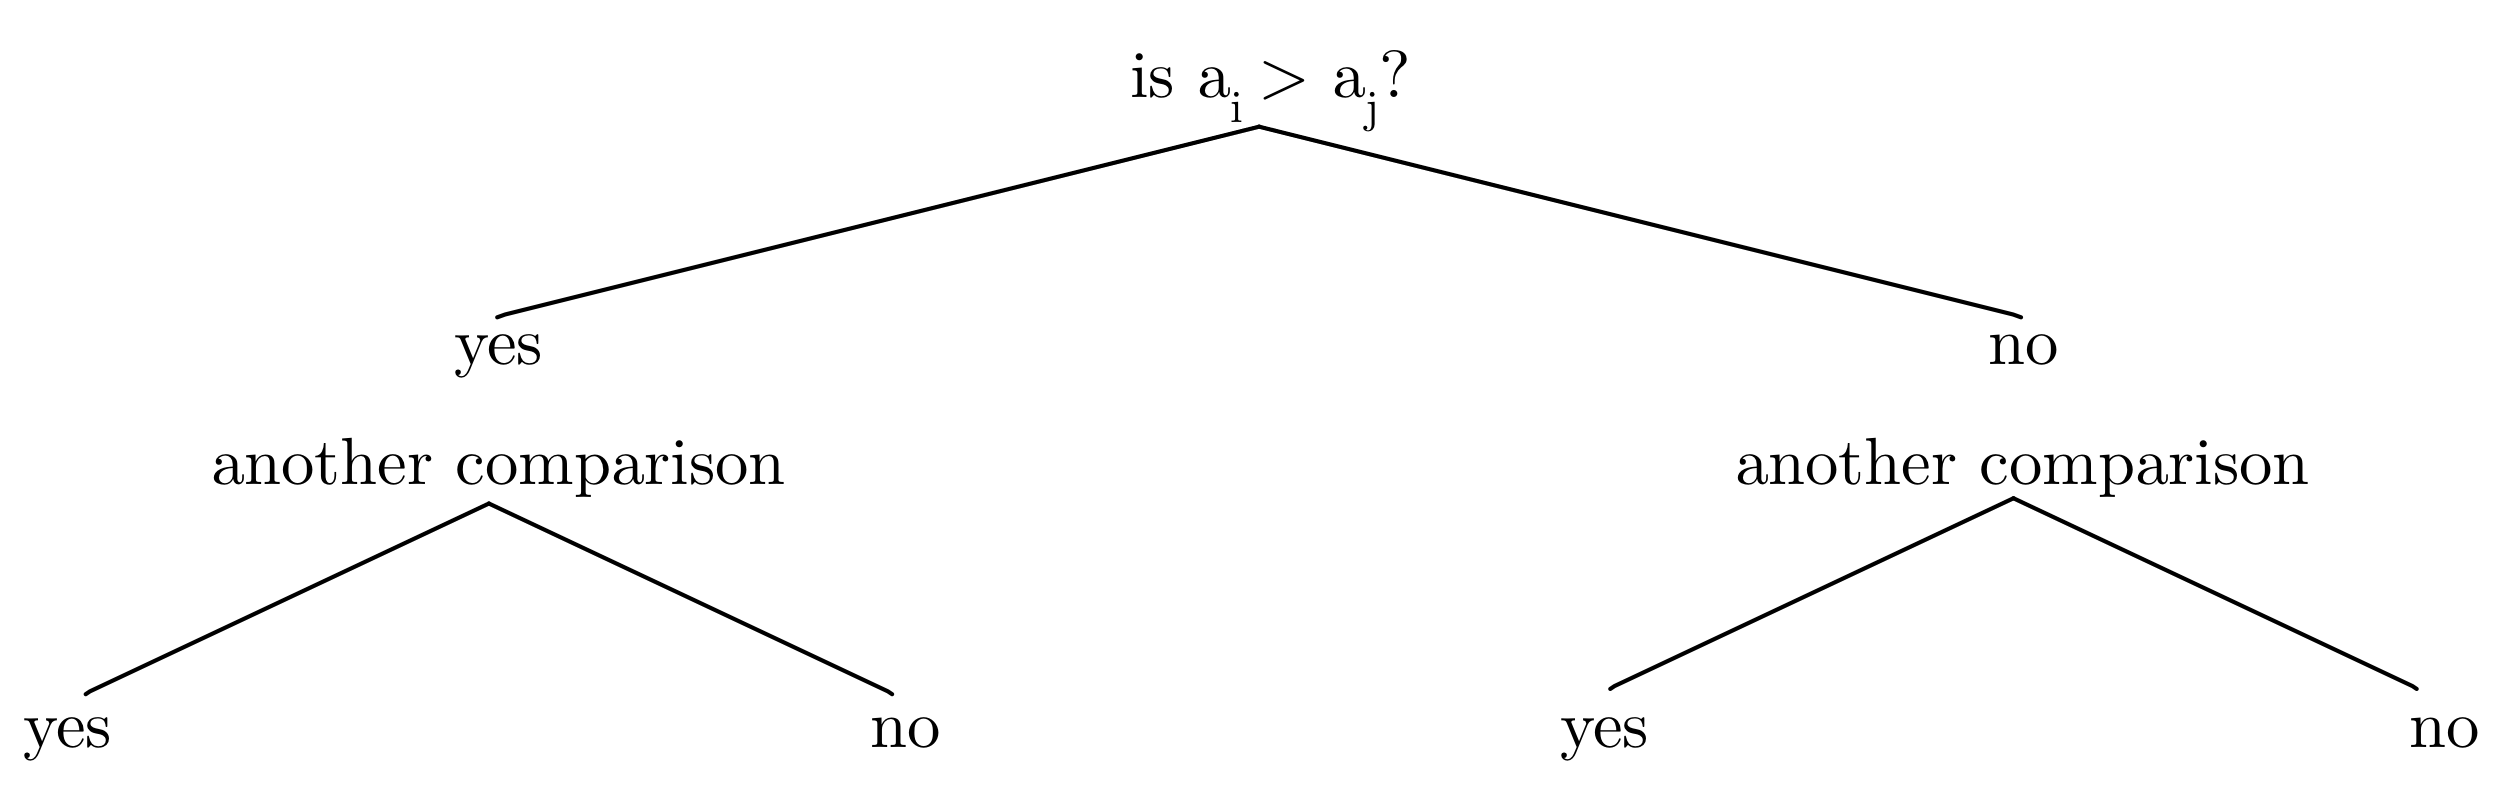
\includegraphics[width=.5\linewidth]{./images/big_o_theta_etc/Decision_tree_comparison_search.png}
\caption{\label{}
Portion of a binary decision tree for a comparison-based sorting algorithm.}
\end{figure*}
Let \(S\) be the set of inputs that are consistent with the answers to comparisons made so far. Initially, \(|S| = n!\). Each comparison splits \(S\) into two groups: those inputs for which the answer is YES and those for which the answer is NO. Each comparison cuts down the size of \(S\) by at most a factor of 2. Since initially the size of \(S\) is \(n!\), and in the end it should be reduced to 1 (one correct solution), the algorithm must make \(log_{2}(n!)\) comparisons.

Since we're looking for a lower bound, Big O notation doesn't apply. For this, Big Omega (\(\Omega\)) is used. Similar to Big O, Big Omega is a way to say that some function \(g(n)\) is always "lower" than the function in question.

\begin{figure*}[htbp]
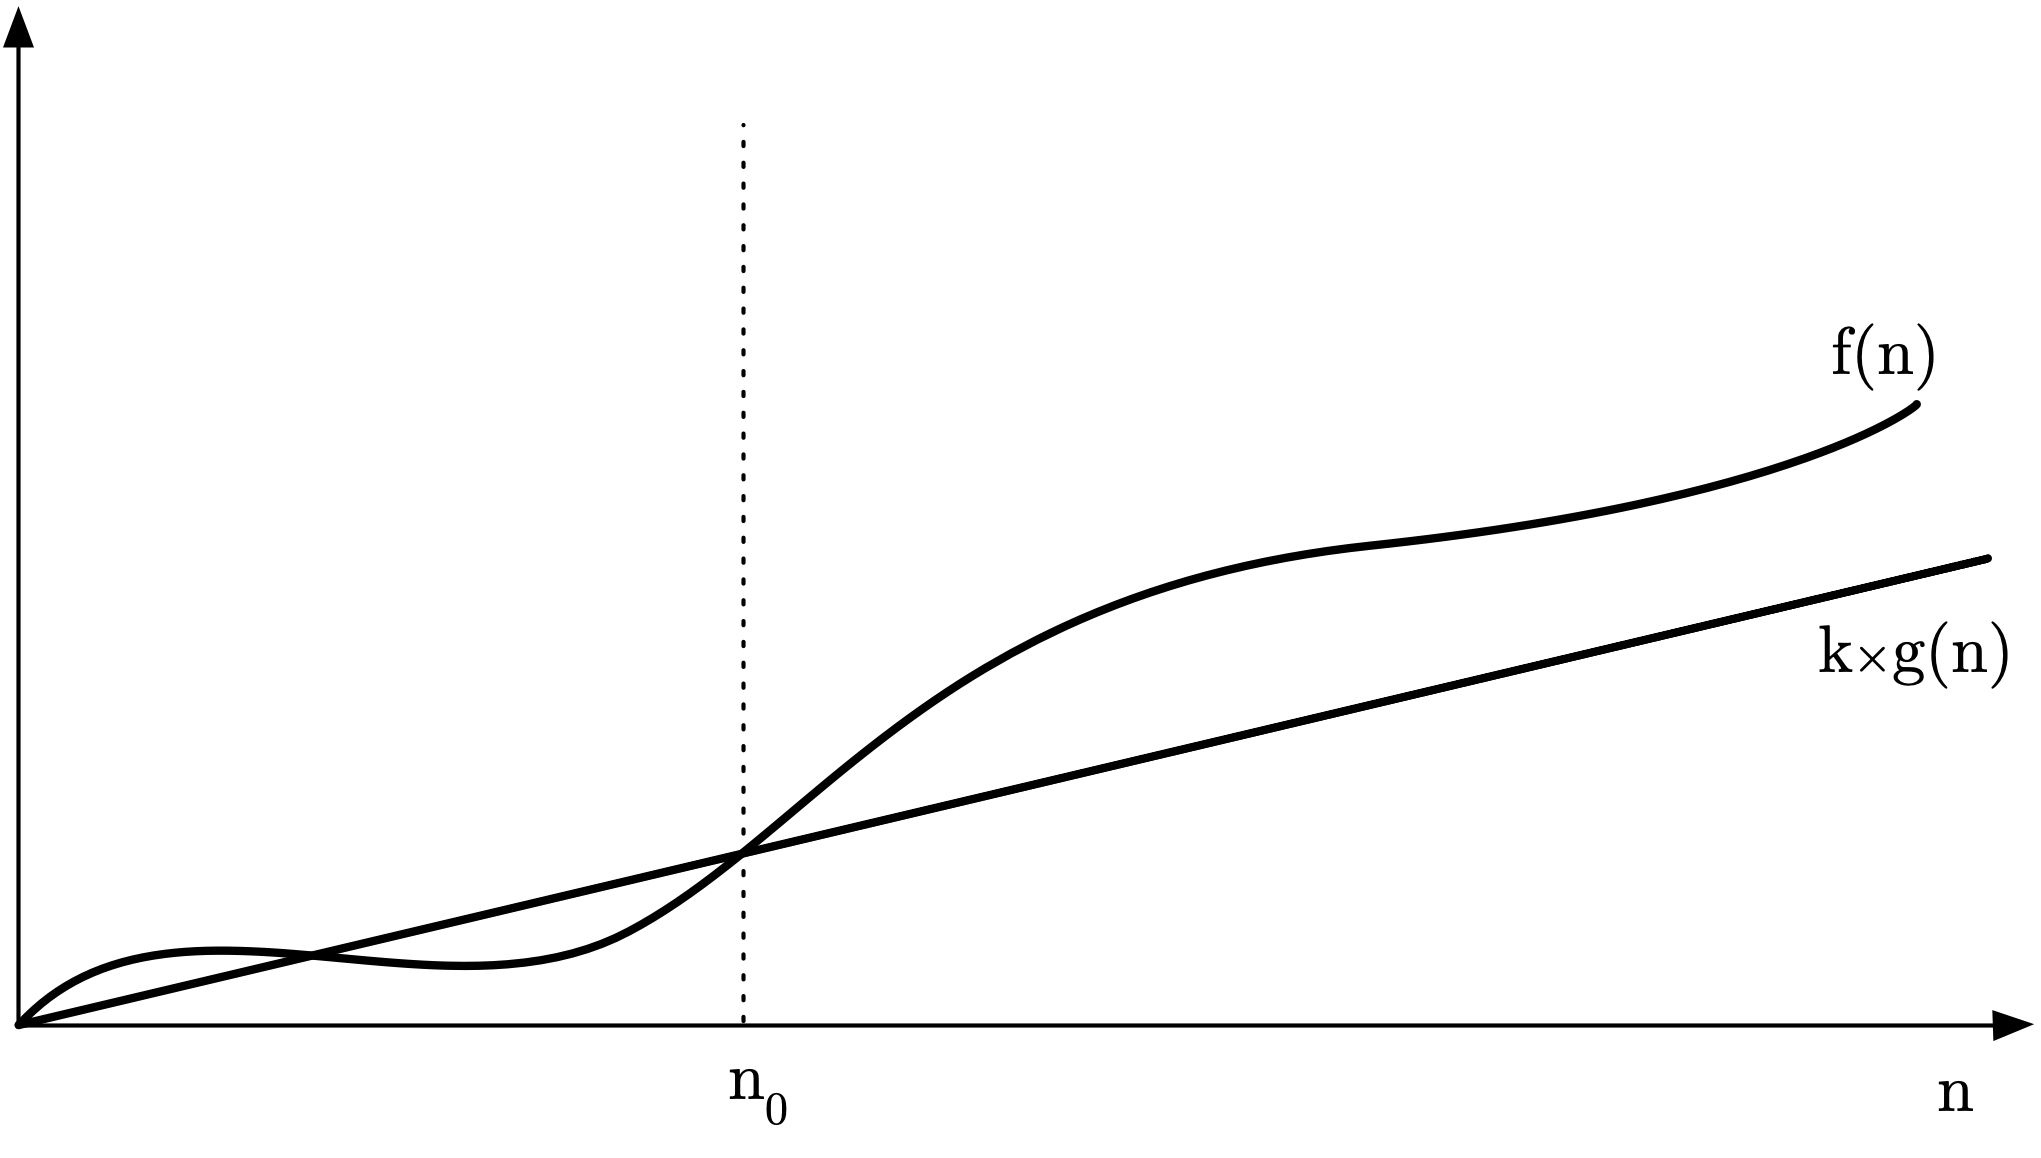
\includegraphics[width=.5\linewidth]{./images/big_o_theta_etc/Big_Omega.png}
\caption{\label{}
Graphs of f(n) and g(n).}
\end{figure*}
$$ log_{2}(n!) = log_{2}(n) + log_{2}(n-1) \textrm{ + ... + } log_{2}(2) $$
$$ = \Omega(n log_{2}n) $$

Because \(log_{2}n\) is so frequent in computer science, number 2 is usually omitted and only \(logn\) is written. So, the lower bound for any comparison-based sorting algorithm is \(\Omega(n logn)\).

Heapsort and Mergesort sorting algorithms have an upper bound of \(\mathcal{O}(nlogn)\) steps. Therefore, they are optimal, as their upper bound is the same as the lower bound for any comparison-based sorting algorithm.
\chapter{Divide and conquer}
\label{sec:orgeaa0a91}
\chapter{Big theta, etc}
\label{sec:org75e19a6}

\part{{\bfseries\sffamily TODO} s}
\label{sec:org3973052}
\chapter{Graphs}
\label{sec:orgae72d43}
\begin{itemize}
\item bridges problem
\item dijkstra's algorithm
\end{itemize}

\chapter{Data structures}
\label{sec:orgedbcf1c}
\begin{itemize}
\item array
\item hash-table
\item linked list
\item tree
\end{itemize}

\chapter{Euclid links}
\label{sec:orgf4b5ddf}
\begin{itemize}
\item \url{https://repl.it/@rakhim/Scratchpad}
\item \url{https://www.youtube.com/watch?v=sCXezzlX7kw}
\item \url{http://www.maths.surrey.ac.uk/hosted-sites/R.Knott/Fibonacci/fibtable.html}
\item \url{https://math.stackexchange.com/questions/2096929/how-to-find-number-of-steps-in-euclidean-algorithm-for-fibonacci-numbers}
\item \url{https://www.math.wustl.edu/\~victor/talks/euclid.pdf}
\item \url{https://ia902505.us.archive.org/18/items/Lecture14/Lecture\%201-4.pdf}
\item \url{https://stackoverflow.com/questions/3980416/time-complexity-of-euclids-algorithm}
\end{itemize}

\chapter{End of book}
\label{sec:org65b24f9}
\begin{itemize}
\item proofs
\item why \(log_{2}(n!)\) comparisons in comparison-based sorting algorithm
\end{itemize}
\end{document}
